


%=================================================================
\documentclass[journal,article,submit,pdftex,moreauthors]{Definitions/mdpi} 


% 若要将本稿件的早期版本作为预印本发布,可使用 “preprints ”作为期刊。发布前将 “提交 ”改为 “接受 ”将删除行号。
%----------
% article
%----------
% submit
%----------
%论文被接受后,编辑部会将 “提交 ”类选项更改为 “接受”。这只会更改首页(例如,期刊的徽标将变得可见)、标题和版权信息。此外,行号将被删除。被录用论文的期刊信息和页码也将由编辑部指定。

%------------------
% moreauthors
%------------------
% 如果只有一位作者,则应使用 “一位作者 ”类别选项。否则,应使用 “更多作者 ”类别选项。
%---------
% pdftex
%---------
% 选项 pdftex 用于 pdfLaTeX。如果(1)使用 LaTeX 和 dvi2pdf(如果使用 eps 数字)或(2)使用 XeLaTeX 进行编译,请移除 “pdftex”。

%=================================================================
% MDPI internal commands - do not modify
\firstpage{1} 
\makeatletter 
\setcounter{page}{\@firstpage} 
\makeatother
\pubvolume{1}
\issuenum{1}
\articlenumber{0}
\pubyear{2024}
\copyrightyear{2024}
%\externaleditor{Academic Editor: Firstname Lastname}
\datereceived{ } 
\daterevised{ } % Comment out if no revised date
\dateaccepted{ } 
\datepublished{ } 
%\datecorrected{} % For corrected papers: "Corrected: XXX" date in the original paper.
%\dateretracted{} % For corrected papers: "Retracted: XXX" date in the original paper.
\hreflink{https://doi.org/} % If needed use \linebreak
%\doinum{}
%\pdfoutput=1 % Uncommented for upload to arXiv.org
%\CorrStatement{yes}  % For updates


%=================================================================
% 在此添加软件包和命令。在我们的类文件中加载了以下软件包:inputenc, calc, indentfirst, fancyhdr, graphicx, epstopdf, lastpage, ifthen, float, amsmath, amssymb, lineno, setspace, enumitem, mathpazo, booktabs, titlesec, etoolbox, tabto, xcolor, colortbl, soul, multirow, microtype, tikz, totcount, changepage, attrib, upgreek, array, tabularx, pbox, ragged2e, tocloft, marginnote, marginfix, enotez, amsthm, natbib, hyperref, cleveref, scrextend, url, geometry, newfloat, caption, draftwatermark, seqsplit
% cleveref: load \crefname definitions after \begin{document}

%=================================================================
% 请使用以下数学环境:Theorem, Lemma, Corollary, Proposition, Characterization, Property, Problem, Example, ExamplesandDefinitions, Hypothesis, Remark, Definition, Notation, Assumption
%% For proofs, please use the proof environment (the amsthm package is loaded by the MDPI class).

%=================================================================
% Full title of the paper (Capitalized)
\Title{A Multi-Scale Feature Fusion Model for Lost Circulation Monitoring Using Wavelet Transform and TimeGAN}

% MDPI internal command: Title for citation in the left column
\TitleCitation{A Multi-Scale Feature Fusion Model for Lost Circulation Monitoring Using Wavelet Transform and TimeGAN}

% Author Orchid ID: enter ID or remove command
\newcommand{\orcidauthorA}{0009-0007-5415-3060} % Add \orcidA{} behind the author's name
%\newcommand{\orcidauthorB}{0000-0000-0000-000X} % Add \orcidB{} behind the author's name

% Authors, for the paper (add full first names)
\Author{Yuan Sun $^{1}$, Jiangtao Wang  $^{1}$ , Ziyue Zhang $^{2}$* , Fei Fan  $^{1}$, Zhaopeng Zhu$^{2}$}

%\longauthorlist{yes}

% MDPI internal command: Authors, for metadata in PDF
\AuthorNames{Yuan Sun, Jiangtao Wang , Ziyue Zhang, Fei Fan, Zhaopeng Zhu}

% MDPI internal command: Authors, for citation in the left column
\AuthorCitation{
Sun, Y.; Wang, J.; Zhang, Z.; Fan, F.; Zhu, Z.
}


% Affiliations / Addresses (Add [1] after \address if there is only one affiliation.)
\address{%
$^{1}$\quad China France Bohai Geoservices Co., Ltd. sunyuan@cfbgc.com(S.Y.)wangjiangt@cfbgc.com (J.W.);fanfei@cfbgc.com(F.F)

$^{2}$ \quad School of Petroleum Engineering, China University of Petroleum, Beijing 102249, China;
2024310189@student.cup.edu.cn(Z.Z.);zhuzp@cup.edu.cn(Z.Z.)\\
}

% Contact information of the corresponding author
\corres{Correspondence:2024310189@student.cup.edu.cn; Tel.: +86-135-1287-2028}
% Current address and/or shared authorship
%\firstnote{Current address: Affiliation.}  % Current address should not be the same as any items in the Affiliation section.
%\secondnote{These authors contributed equally to this work.}
% The commands \thirdnote{} till \eighthnote{} are available for further notes

%\simplesumm{} % Simple summary

%\conference{} % An extended version of a conference paper
% Abstract (Do not insert blank lines, i.e. \\) 
\abstract{The issue of lost circulation represents a significant challenge in drilling, given its potential to impede both safety and efficiency.    The traditional monitoring model is hindered by the presence of noise and the complexity of temporal fluctuations in lost circulation data, resulting in suboptimal performance with regard to accuracy and generalisation ability.    This, in turn, complicates the adaptation of the model to diverse working conditions.   To address these limitations, this study proposes a multi-scale feature fusion model based on wavelet transform and TimeGAN.    Wavelet transform enhances the features of time series data, while TimeGAN (Time Series Generative Adversarial Network) excels in generating realistic time series and augmenting scarce or missing data.    This model leverages convolutional network feature extraction and integrates features via a multi-scale feature fusion module to investigate correlations among different features.   Consequently, it effectively mitigates the overfitting issue caused by limited drilling loss samples.  The experimental findings demonstrate that the multi-scale feature fusion model proposed in this study enhances the accuracy by 8.8\% , reduces the leakage rate and false alarm rate by 12.4\%  and 6.2\% , respectively, and attains a test set accuracy of 93.8\%  and an accuracy of 95.1\%  in the lost circulation identification task in comparison to the unoptimized model.    The method outlined in this study provides reliable technical support for the monitoring of lost circulation risk, thereby contributing to the enhancement of safety and efficiency in the drilling process.}

% Keywords
\keyword{Wavelet transform; TimeGAN; multi-scale feature fusion;  lost circulation risk} 

% The fields PACS, MSC, and JEL may be left empty or commented out if not applicable
%\PACS{J0101}
%\MSC{}
%\JEL{}

%%%%%%%%%%%%%%%%%%%%%%%%%%%%%%%%%%%%%%%%%%
% Only for the journal Diversity
%\LSID{\url{http://}}

%%%%%%%%%%%%%%%%%%%%%%%%%%%%%%%%%%%%%%%%%%
% Only for the journal Applied Sciences
%\featuredapplication{Authors are encouraged to provide a concise description of the specific application or a potential application of the work. This section is not mandatory.}
%%%%%%%%%%%%%%%%%%%%%%%%%%%%%%%%%%%%%%%%%%

%%%%%%%%%%%%%%%%%%%%%%%%%%%%%%%%%%%%%%%%%%
% Only for the journal Data
%\dataset{DOI number or link to the deposited data set if the data set is published separately. If the data set shall be published as a supplement to this study, this field will be filled by the journal editors. In this case, please submit the data set as a supplement.}
%\datasetlicense{License under which the data set is made available (CC0, CC-BY, CC-BY-SA, CC-BY-NC, etc.)}

%%%%%%%%%%%%%%%%%%%%%%%%%%%%%%%%%%%%%%%%%%
% Only for the journal Toxins
%\keycontribution{The breakthroughs or highlights of the manuscript. Authors can write one or two sentences to describe the most important part of the paper.}

%%%%%%%%%%%%%%%%%%%%%%%%%%%%%%%%%%%%%%%%%%
% Only for the journal Encyclopedia
%\encyclopediadef{For entry manuscripts only: please provide a brief overview of the entry title instead of an abstract.}

%%%%%%%%%%%%%%%%%%%%%%%%%%%%%%%%%%%%%%%%%%
% Only for the journal Advances in Respiratory Medicine
%\addhighlights{yes}
%\renewcommand{\addhighlights}{%

%\noindent This is an obligatory section in “Advances in Respiratory Medicine”, whose goal is to increase the discoverability and readability of the article via search engines and other scholars. Highlights should not be a copy of the abstract, but a simple text allowing the reader to quickly and simplified find out what the article is about and what can be cited from it. Each of these parts should be devoted up to 2~bullet points.\vspace{3pt}\\
%\textbf{What are the main findings?}
% \begin{itemize}[labelsep=2.5mm,topsep=-3pt]
% \item First bullet.
% \item Second bullet.
% \end{itemize}\vspace{3pt}
%\textbf{What is the implication of the main finding?}
% \begin{itemize}[labelsep=2.5mm,topsep=-3pt]
% \item First bullet.
% \item Second bullet.
% \end{itemize}
%}

%%%%%%%%%%%%%%%%%%%%%%%%%%%%%%%%%%%%%%%%%%
         \begin{document}
\section*{Abbreviations}
\begin{enumerate}
    \item BP: Back Propagation
    \item GAN: Generative Adversarial Network
    \item SPP: Standpipe Pressure
    \item TPIT: Total Pool Volume
    \item MFO: Outlet Flow Rate
    \item MFI: Inlet Flow Rate
    \item GRU: Gated Recurrent Unit
    \item WT: Wavelet Transform
    \item TimeGAN: Time Series Generative Adversarial Network
\end{enumerate}
%%%%%%%%%%%%%%%%%%%%%%%%%%%%%%%%%%%%%%%%%%
\section{Introduction}

Conventional oil and gas resources are a subject of continuous development, and the oil and gas exploration and development industry is gradually expanding towards complex oil and gas fields such as unconventional, deep and deep sea, which are rich in resources. The presence of complex oil and gas formations, characterised by high temperature and pressure, intricate layers, and vulnerability to instability, gives rise to significant and often unacknowledged lost circulation risks. The challenge of identifying these risks is further compounded by the presence of data noise, real-time fluctuations, and nonlinear mapping relationships, which contribute to the complexity of the situation. If these risks are not detected in a timely manner, resulting in processing lag, the consequences can be severe, including the potential for malignant leakage and well blowout accidents. Consequently, the accurate and effective monitoring of lost circulation risk is of paramount importance for ensuring the safety and efficiency of drilling operations.

At present, the field of lost circulation diagnostics can be divided into two broad categories: traditional methods and methods based on intelligent technologies. Engineers reliant upon traditional methods utilise sensor equipment to monitor real-time fluctuations of key parameters in the drilling process, in order to make judgements regarding lost circulation. However, such traditional methods are limited by the measurement accuracy of the sensors and the experience level of the engineers; moreover, the accuracy and timeliness of these methods is often insufficient. In recent years, with the advent of deep learning technology, the focus of research in lost circulation diagnosis has shifted towards monitoring methods based on intelligent algorithms. For instance, in 2016, Simeng Han et al.\cite{simeng2016}  explored real-time early warning methods for drilling overflows and constructed a real-time early warning model based on on the sign parameters through BP neural networks.In 2019, Liu Biao's team\cite{liubiao2019} upgraded the lost circulation early warning system with support vector regression technology.In 2023, Yan Yan's team\cite{yandan2023} applied the risk trend line method to improve the early warning capability of drilling overflow and lost circulation risk. In the same year, Zheng Zhuo's team \cite{zhengzhuo2023}utilised the XGBoost algorithm to construct a lost circulation warning model for the Bohai Oilfield, achieving an accuracy of 87\%.Sun Weifeng's team \cite{sunweifeng2023} proposed a lost circulation monitoring method based on DCC-LSTM. DCC-LSTM (Dynamic Conditional Correlation Long Short-Term Memory network) is an advanced time series prediction model that effectively captures the dynamic correlations between multidimensional data, making it particularly suitable for complex data analysis in lost circulation monitoring. They improved the accuracy of well leakage incident prediction to 75\% while simultaneously reducing the false alarm rate.These methodologies are adept at handling substantial data volumes and identifying anomalies through automated models. Nevertheless, the inability of features to adequately characterise the lost circulation state under the prevailing data conditions, in conjunction with the paucity of valid lost circulation samples, constitute the primary constraints on the efficacy of intelligent models.

In the field of lost circulation detection, effective lost circulation data features typically contain complex information in both the time and frequency domains. However, existing models have limited capabilities in extracting these complex features, and the performance of intelligent models is significantly constrained by the scarcity of valid lost circulation samples. Therefore, this study proposes a multiscale feature fusion model that combines wavelet transform and TimeGAN. The model not only extracts multi-scale time-series features from lost circulation data using wavelet transform but also generates new samples with TimeGAN to address the issue of insufficient samples. The optimal feature fusion strategy is obtained through the multiscale feature fusion module, which enhances both diagnostic accuracy and stability. This method not only overcomes the data scarcity problem in lost circulation detection but also thoroughly explores the temporal and frequency features in lost circulation data, providing an efficient and accurate solution for monitoring lost circulation risks while reducing reliance on a large amount of labeled lost circulation data.
%%%%%%%%%%%%%%%%%%%%%%%%%%%%%%%%%%%%%%%%%%
\section{Methodology}
\subsection{Wavelet Transform}

Wavelet Transform (WT) is a tool for analysing signals in the time and frequency domains \cite{Grossmann1984}, which is widely used in fields such as noise removal and pattern recognition. Its basic formula is:
\[{{W}_{\psi }}(a,b)=\frac{1}{\sqrt{|a|}}\mathop{\int }_{-\infty }^{+\infty }f(t)\psi (\frac{t-b}{a})dt\quad (1)\]

where $W\psi(a, b)$ are the wavelet coefficients, $f(t)$ is the signal to be analysed, $\psi$ is the mother wavelet function, and $a$ and $b$ denote the scale and translation parameters, respectively.
The wavelet transform method is utilised to process the original feature signal, with the signal initially decomposed into 'low frequency approximation' and 'high frequency details'. This is followed by a further decomposition of the 'low frequency approximation' and 'high frequency details' into 'low frequency approximation' and 'high frequency details'. A subsequent decomposition of the resultant part of the last decomposition is then performed into 'low-frequency approximation' and 'high-frequency details', with each part of the decomposition subdivided individually until each part of the decomposition is limited to a single point. The 'high-frequency details' part is not decomposed, and the decomposition steps are illustrated in Figure ~\ref{fig:Wavelet Transform}. The application of wavelet transform facilitates the division of the signal into multiple scales, thereby enabling the analysis of the information of the target signal in each frequency band with greater precision and facilitating a comprehensive exploration of the intrinsic law of the signal.

\begin{figure}[h]
    \centering
    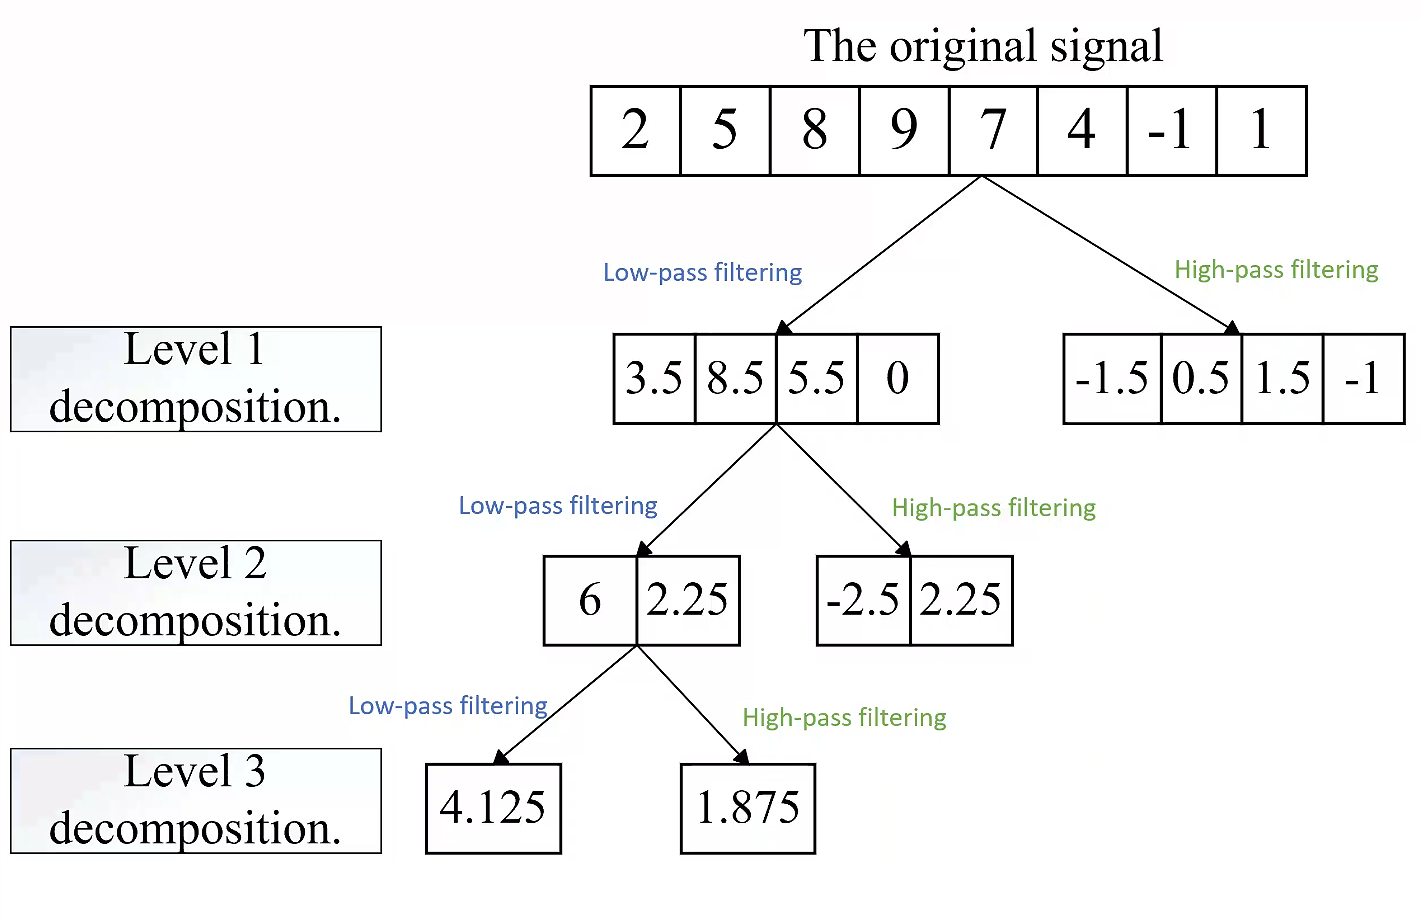
\includegraphics[width=0.75\linewidth]{图片/小波变换.png}
    \caption{Schematic of wavelet multilevel decomposition}
    \label{fig:Wavelet Transform}
\end{figure}


%%%%%%%%%%%%%%%%%%%%%%%%%%%%%%%%%%%%%%%%%%
\subsection{TimeGAN }

The training process of GAN is an adversarial process, where the generator and the discriminator compete with each other in a game. In this game, the generator tries to generate more and more realistic fake data, while the discriminator tries to distinguish between real data and fake data as accurately as possible. The enhancement of TimeGAN \cite{Yoon2019} is attributable to its comprehension of two pivotal characteristics of temporal data: namely, the static features, which remain constant over time, and the temporal features, which undergo change over time.The TimeGAN network comprises four constituent elements: the embedding function, the recovery function, the sequence generator, and the sequence discriminator. The configuration of this network is illustrated in Figure \ref{fig:timegan}.  


\begin{figure}[h]
    \centering
    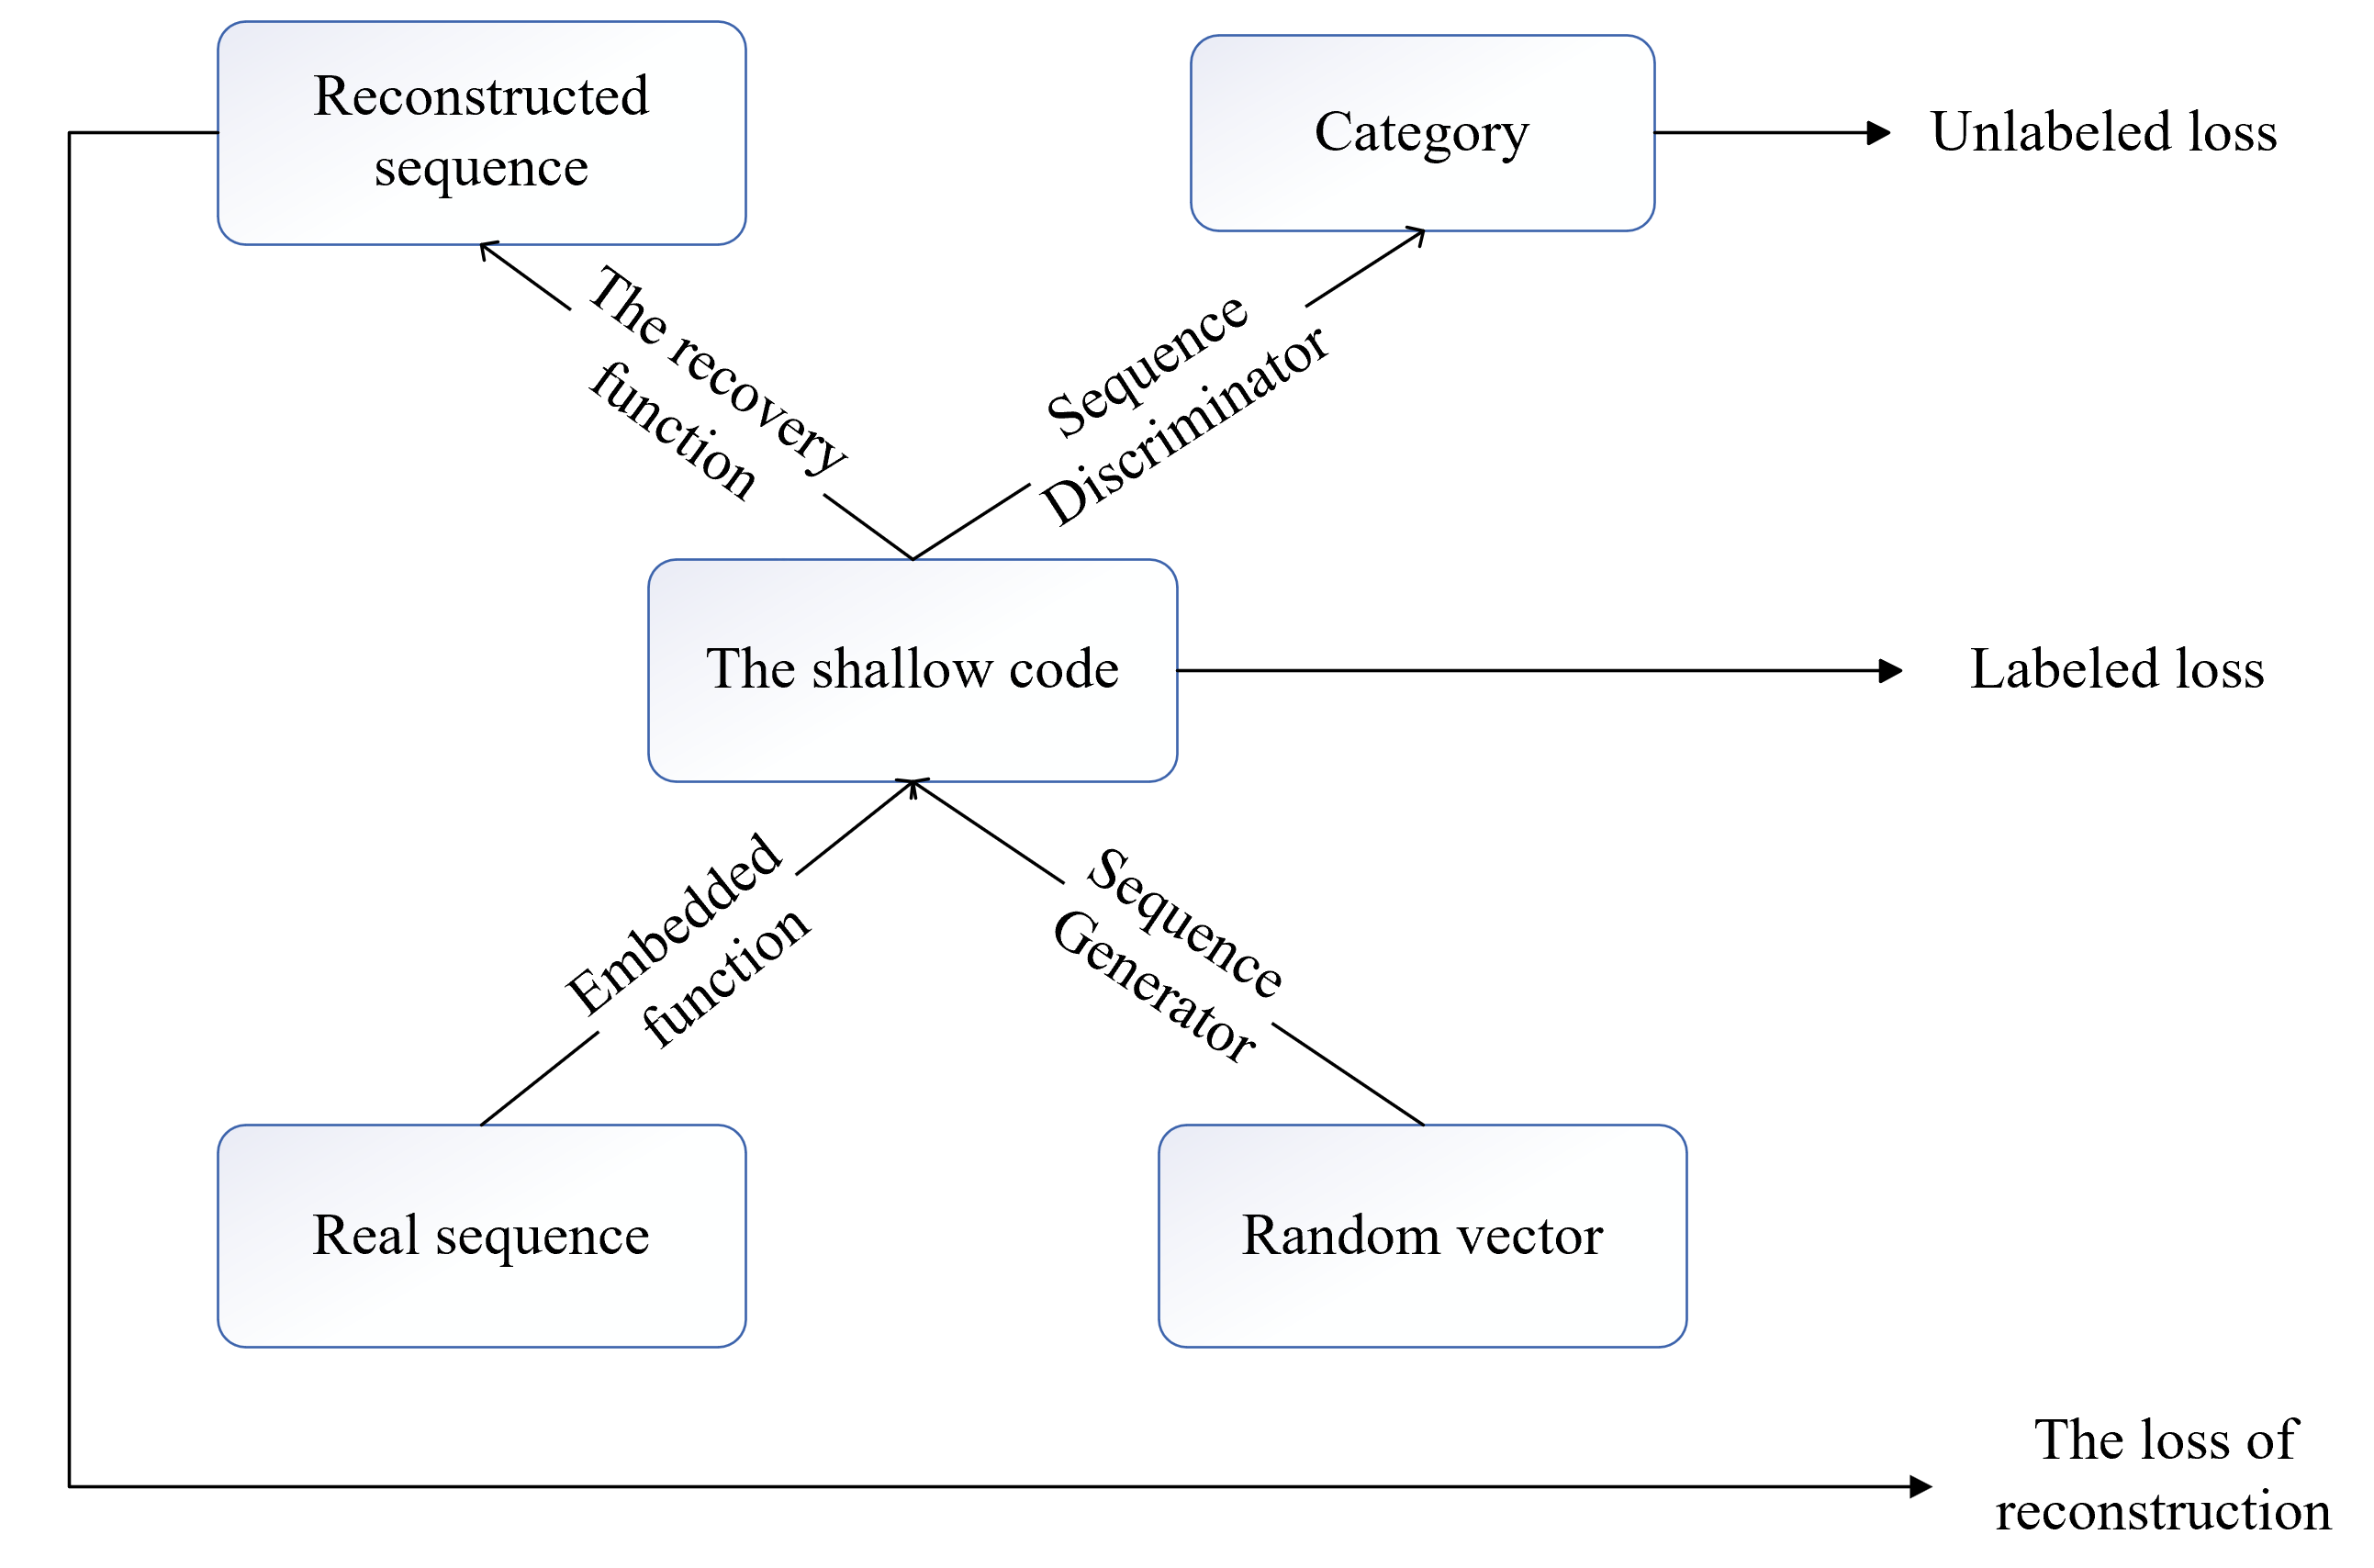
\includegraphics[width=0.75\linewidth]{图片/timegan组成.png}
    \caption{TimeGAN Components}
    \label{fig:timegan}
\end{figure}

The auto-coding component of TimeGAN is capable of realising the inverse mapping between feature space and potential space, and can reconstruct the data according to the potential static and temporal features of the real data. The mathematical expressions for the reconstruction loss function \({{I}_{R}}\), the unsupervised loss function \({{I}_{u}}\) and the additional supervised loss function \({{I}_{s}}\) during training are as follows.

$$ I _ { R } = E _ { S , X _ { 1: T - P } } \left[ | S - \tilde { S } | | _ { 2 } + \sum _ { t } | | X _ { t } - \tilde { X } _ { t } | | _ { 2 } \right]\quad (2)$$
$$ I _ { U } = E _ { S , X _ {1: T- P } } \left[ \log y _ { s } + \sum _ { t } \log y _ { t } \right] + E _ { S , X _ { 1: T - \widehat { p } } } \left[ \log ( 1 - \widehat { y } _ { s } ) + \sum _ { t } \log ( 1 - \widehat { y } _ { t } ) \right]\quad (3)$$
$$ I _ { S } = E _ { S , X _ { 1: T - P } } \left[ \sum _ { t } | | h _ { t } - g _ { x } ( h _ { S } , h _ { t - 1 } , z _ { t } ) | | _ { 2 } \right]\quad (4)$$

where \({{\widetilde{S}}}\) and \({{\widetilde{X}}_{1:T}}\) denote the static and temporal feature vectors of the generated data,  \({S}\) and \({X}_{1:T}\) denote the static and temporal feature vectors of the real data,  \({h}_{s}\) and  \({h}_{1:T}\) denote the static and temporal feature vectors of the latent layer feature space, \({{\widehat{y}}_{s}}\) and  \({{\widehat{y}}_{1:T}}\) denote the discriminator's discriminant values for the static and temporal feature vectors.
%%%%%%%%%%%%%%%%%%%%%%%%%%%%%%%%%%%%%%%%%%
\subsection{Multi-scale feature fusion neural network structure }

The core structure of the network is divided into three parts: a feature extraction module constructed from a convolutional neural network, a feature fusion module for multi-scale feature fusion, and a detection classifier consisting of a fully connected layer \cite{zhaohongyu2023}. The input features of the network include expanded lost circulation data and multiple features after wavelet transform.

The initial extraction of features is accomplished through the utilisation of the larger convolution of the convolution kernel, thereby facilitating the filtration of noise interference in the time series data \cite{meizhou2024}. The initial processing and feature extraction of the input data is executed by the feature extraction backbone network. In comparison with the conventional feature extraction network, the parallel feature extraction approach has the capacity to enhance the feature extraction capability of the model without an increase in complexity\cite{lishutao2018}.

As the various evaluation factors contain rich and complex information, the multi-scale feature fusion model for lost circulation prediction, based on wavelet transform and TimeGAN, extracts feature information through a single scale. This results in insufficient feature mining and inaccurate predictions of lost circulation. To address these limitations, a multi-scale feature fusion model has been developed, as illustrated in Figure ~\ref{fig:Multi-scale cross-feature fusion module}.

\begin{figure}[H]
    \centering
    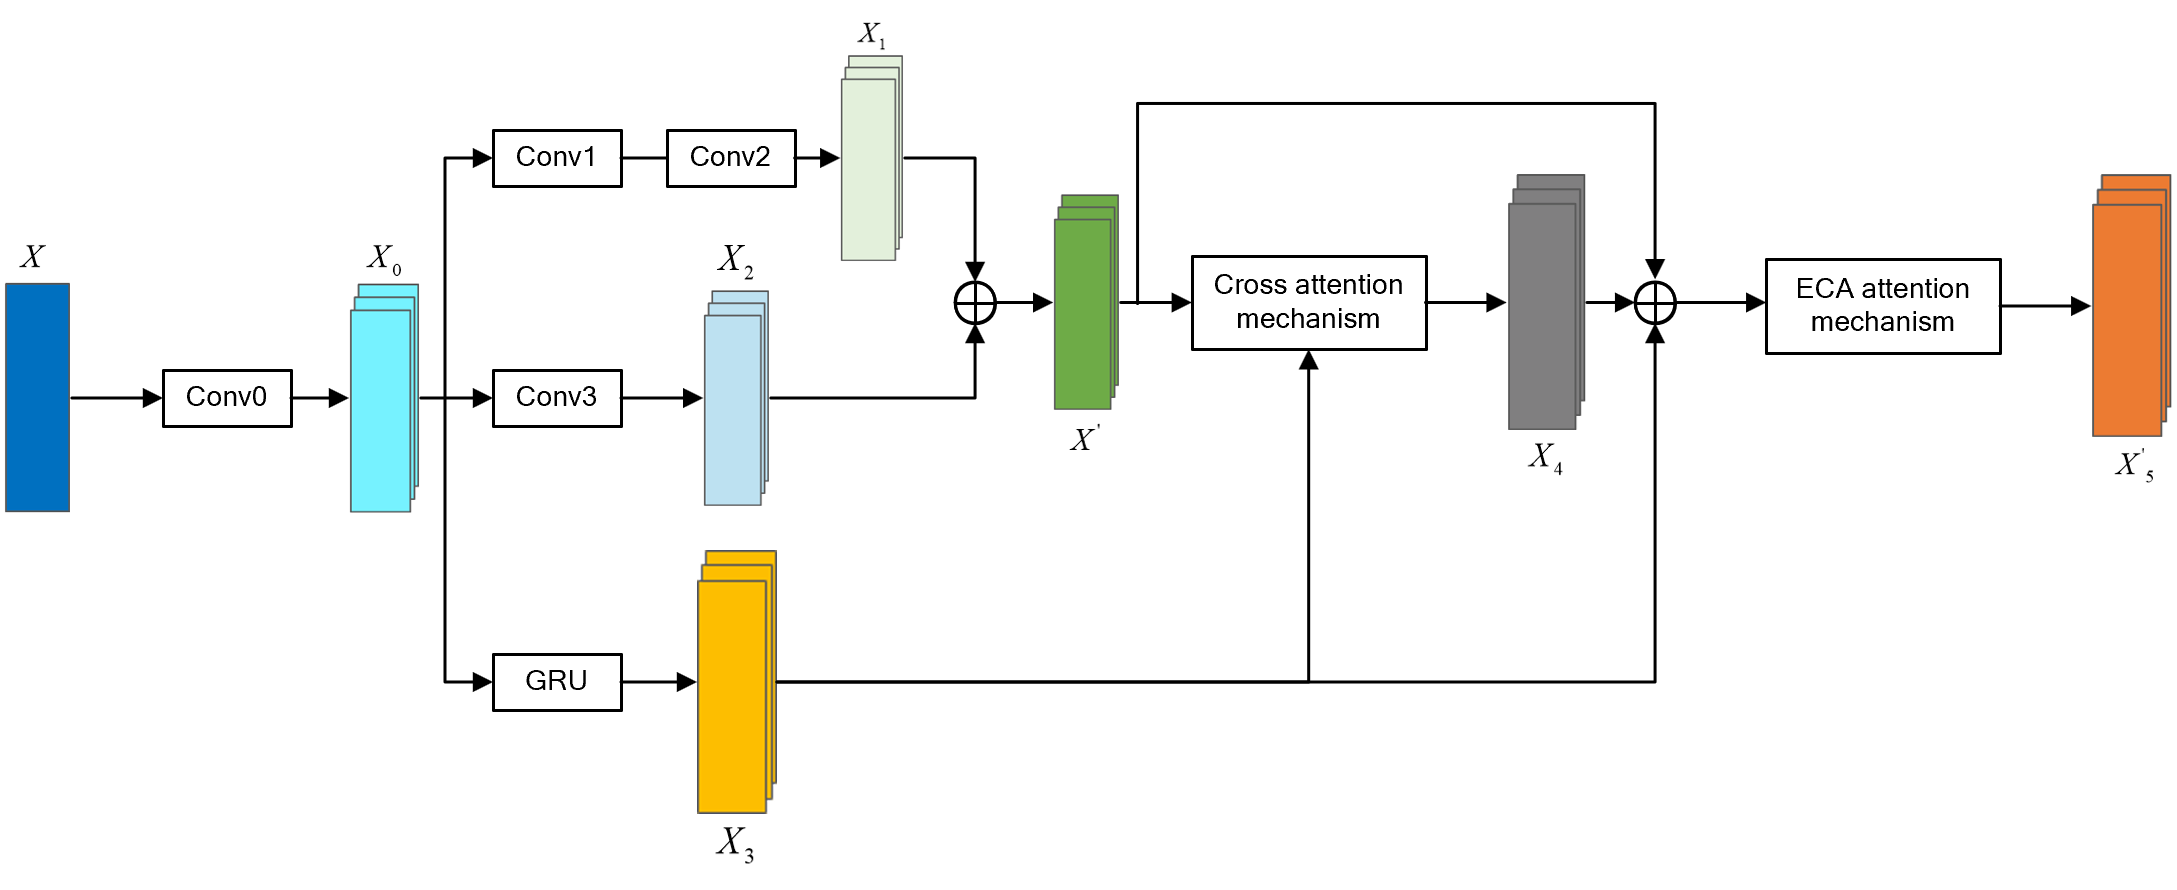
\includegraphics[width=0.75\linewidth]{图片/多尺度特征注意力.png}
    \caption{Multi-scale cross-feature fusion module}
    \label{fig:Multi-scale cross-feature fusion module}
\end{figure}


Subsequently, multi-scale feature extraction is performed on the features that have been obtained following the initial extraction. Local temporal feature extraction of the signal is primarily performed using a convolutional layer, and the long time-dependent features of the signal are captured using a gated loop unit, as illustrated in Equations (5) through (7).
\[{{X}_{1}}=\sigma ({{W}_{2}}(\sigma ({{W}_{1}}({{X}_{0}}+{{b}_{1}}))+{{b}_{2}})\quad (5)\]
	\[{{X}_{2}}=\sigma ({{W}_{3}}({{X}_{0}})+{{b}_{3}})\quad (6)\]
	\[{{X}_{3}}=\sigma ({{f}_{GRU}}({{X}_{0}}))\quad (7)\]

where $\sigma$ denotes the ReLU activation function; \({{W}_{1}}\), \({{W}_{2}}\),  \({{W}_{3}}\) denote the weight matrices corresponding to the convolutions Convl, Conv2, and Conv3, respectively; \({{b}_{1}}\), \({{b}_{2}}\), \({{b}_{3}}\) denote the bias values corresponding to the above convolutions, respectively; and \({{f}_{GRU}}\) denotes the signal input into the gated loop unit.

Each layer uses the attention mechanism to dynamically adjust the feature weights to achieve adaptive allocation of the importance of different features. Specifically, the multi-layer fusion module fuses the expanded lost circulation data and wavelet transformed features at different levels, highlighting key information and suppressing redundant or irrelevant features through the attention mechanism.

For different scales of local time features and long time dependent features, the local time features are summed to get X' and cross attention is calculated with \({{X}_{3}}\) to obtain the fusion feature information. The process of cross-attention mechanism is shown in Fig. \ref{fig:Cross-attention mechanism}.

\begin{figure}[h]
    \centering
    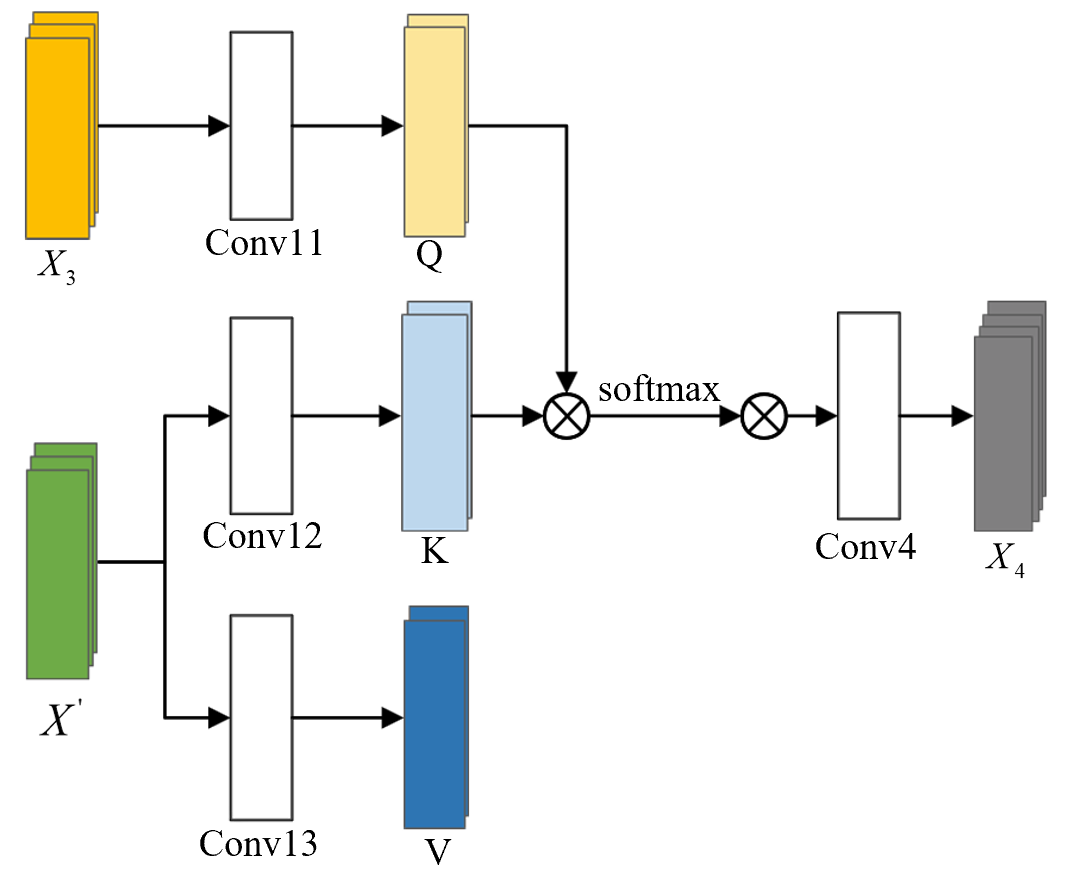
\includegraphics[width=0.75\linewidth]{图片/交叉注意力机制.png}
    \caption{Cross-attention mechanism}
    \label{fig:Cross-attention mechanism}
\end{figure}
The multi-scale cross-feature fusion module is a sophisticated system that extracts local features at multiple scales through the use of convolution kernels at varying scales. In addition, it extracts global features and dependencies in the time series through the implementation of gated recurrent units (GRUs). Ultimately, the module performs feature fusion through the utilisation of the cross-attention mechanism. The feature extraction of local and global features at different scales is an effective method of obtaining a more comprehensive feature representation, which in turn improves the accuracy of fault diagnosis.

Following the acquisition of the enhanced features, these are input into the fully connected layer for the prediction of target information. The detection classifier outputs the probability of lost circulation occurring through the fully connected layer, and the output result is a binary classified lost circulation probability between 0 and 1. Regarding the loss function, the error is calculated using the mean square error, and the output well leakage probability is used as binary cross-entropy. The entire convolutional neural network structure is shown in Fig. \ref{fig:Multi-layer dynamic feature weight neural network structure}.
\begin{figure}[h]
    \centering
    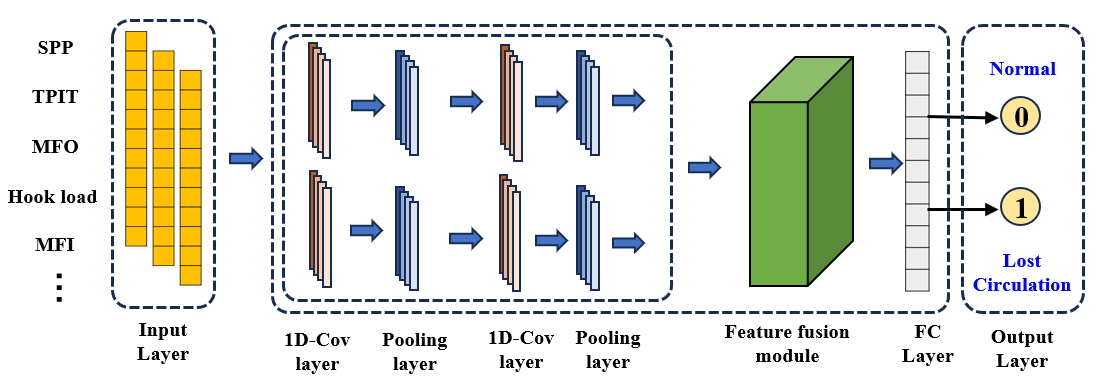
\includegraphics[width=0.75\linewidth]{图片/多尺度融合网络.png}
    \caption{Multi-layer dynamic feature weight neural network structure}
    \label{fig:Multi-layer dynamic feature weight neural network structure}
\end{figure}

%%%%%%%%%%%%%%%%%%%%%%%%%%%%%%%%%%%%%%%%%%
\section{Data Processing}
\subsection{Feature selection}

In this study, the Spearman correlation coefficient method is utilised to optimise the feature set selection process, with consideration given to the data characteristics and computational efficiency.

The method is particularly well-suited to non-normally distributed data.The formula for calculating the Spearman correlation coefficient is as follows:
\[{{r}_{s}}=1-\frac{6\sum\limits_{i=1}^{n}{d_{i}^{2}}}{n\left( {{n}^{2}}-1 \right)}\quad (8)\]

Where,\({{r}_{s}}\) is the final Spearman correlation coefficient value taken by the two variables,\(n\) is the number of data in the variable, and  \(d_{i}^{2}\) is the square of the difference in the rank order of the data of the two variables.


In this study, the Spearman correlation coefficient between each characteristic parameter and the lost circulation label is calculated, and the results are shown in Fig.  \ref{fig:Characteristic correlation coefficient calculation results}

\begin{figure}[h]
    \centering
    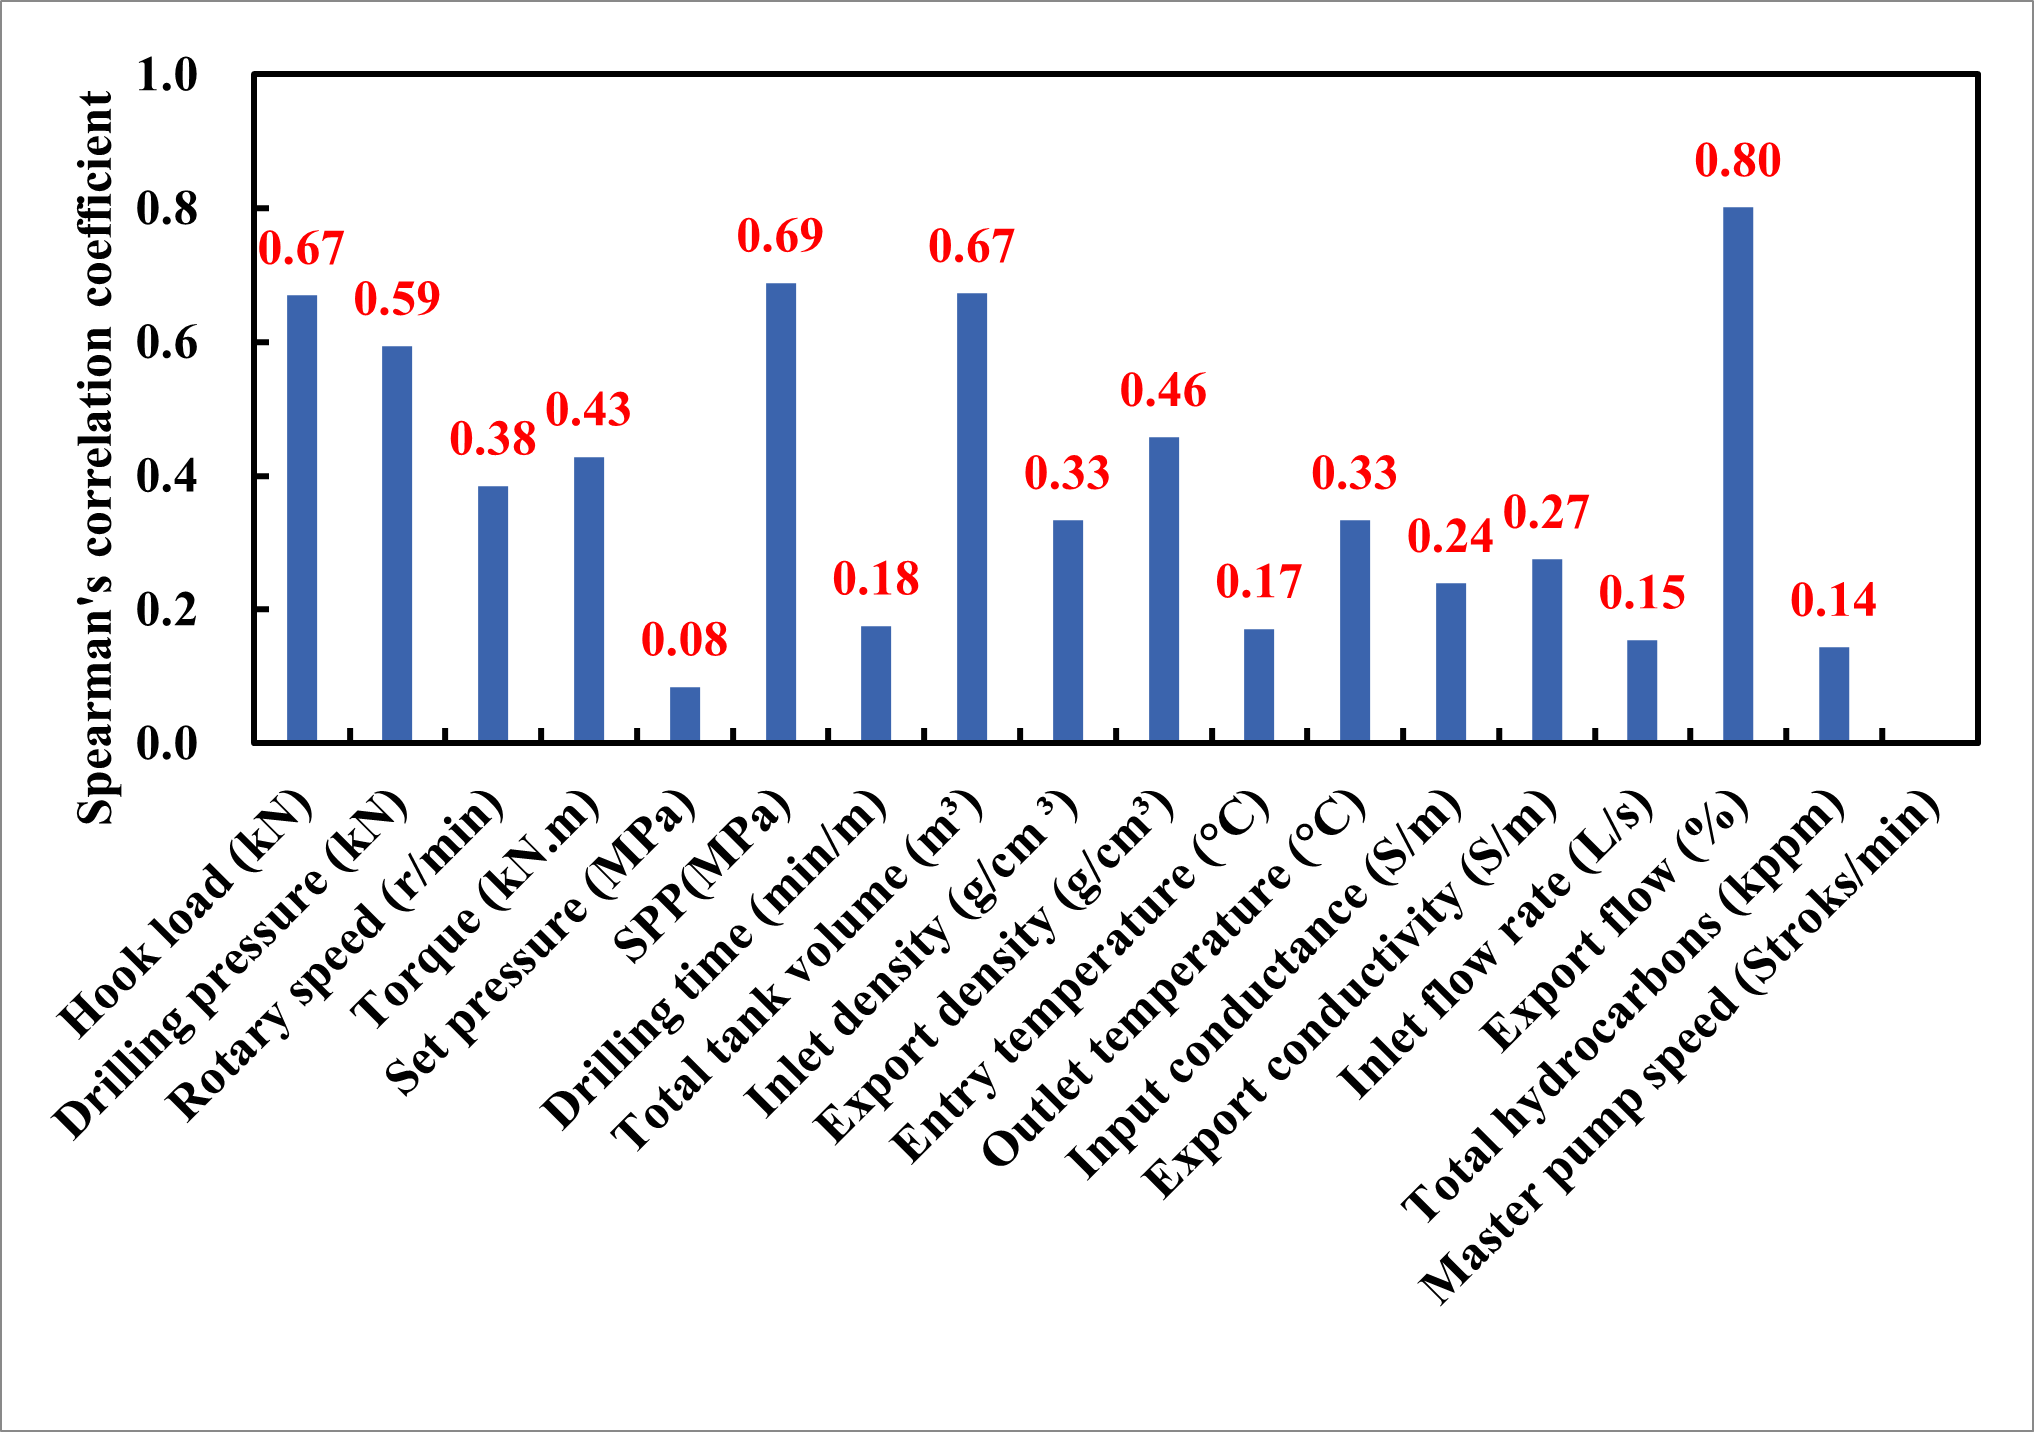
\includegraphics[width=0.75\linewidth]{图片/spearman.png}
    \caption{Characteristic correlation coefficient calculation results}
    \label{fig:Characteristic correlation coefficient calculation results}
\end{figure}

Following a thorough examination of the available domain knowledge, in conjunction with the analysis of expert experience and feature preference, a total of seven parameters were selected as the input features for the intelligent model. Hook load, drilling pressure, torque, riser pressure, TPIT, outlet density and MFO. It was determined that MFO, SPP and TPIT exhibited a high correlation with lost circulation labelling. Furthermore, these parameters were found to be consistent with field engineering practice and expert experience.

%%%%%%%%%%%%%%%%%%%%%%%%%%%%%%%%%%%%%%%%%%
\subsection{Data cleaning}

This study uses time series data from 13 wells in real drilling sites of offshore oil fields in China, with a data acquisition interval of 5 seconds, totaling over 300,000 normal data points and more than 5,000 lost circulation data points.The raw data contains anomalies and missing values. In order to screen the abnormal values, this study adopts the improved sliding window 3 \(\sigma\) method and sets the appropriate window size to avoid misjudging the normal data. The outliers are replaced with null values, which are subsequently filled by spline interpolation to preserve the overall trend of the data. The data were smoothed and filtered using the average of the current point and the previous 99 points to smooth each data point, with the aim of reducing noise and improving data quality. Finally, the maximum-minimum normalisation method was used to dimensionless the data, with the intention of shortening the model training time and reducing overfitting. The relevant formula (9) is as follows:
$$ x _ { s c a l e } = \frac { x - x _ { m i n } } { x _ { m a x } - x _ { m i n } }\quad (9)$$
where x is the data sample, \({{x}_{scale}}\) is the normalised value of \({{x}}\) , and \({{x}_{max}}\)  and \({{x}_{min}}\)  are the maximum and minimum values of the variable \({{x}}\)
%%%%%%%%%%%%%%%%%%%%%%%%%%%%%%%%%%%%%%%%%%
\subsection{Sample construction}

In this study, the sliding window method is used to construct fixed-length  lost circulation time series samples, as shown in Figure\ref{fig:Time series sample construction based on sliding window method} . Under the premise of maximising the use of data, the window sliding step is set to 1, and the window length can be adjusted according to the modelling effect. In order to ensure that the sample has effective features, the window length is usually not less than 30 data points.

\begin{figure}[h]
    \centering
    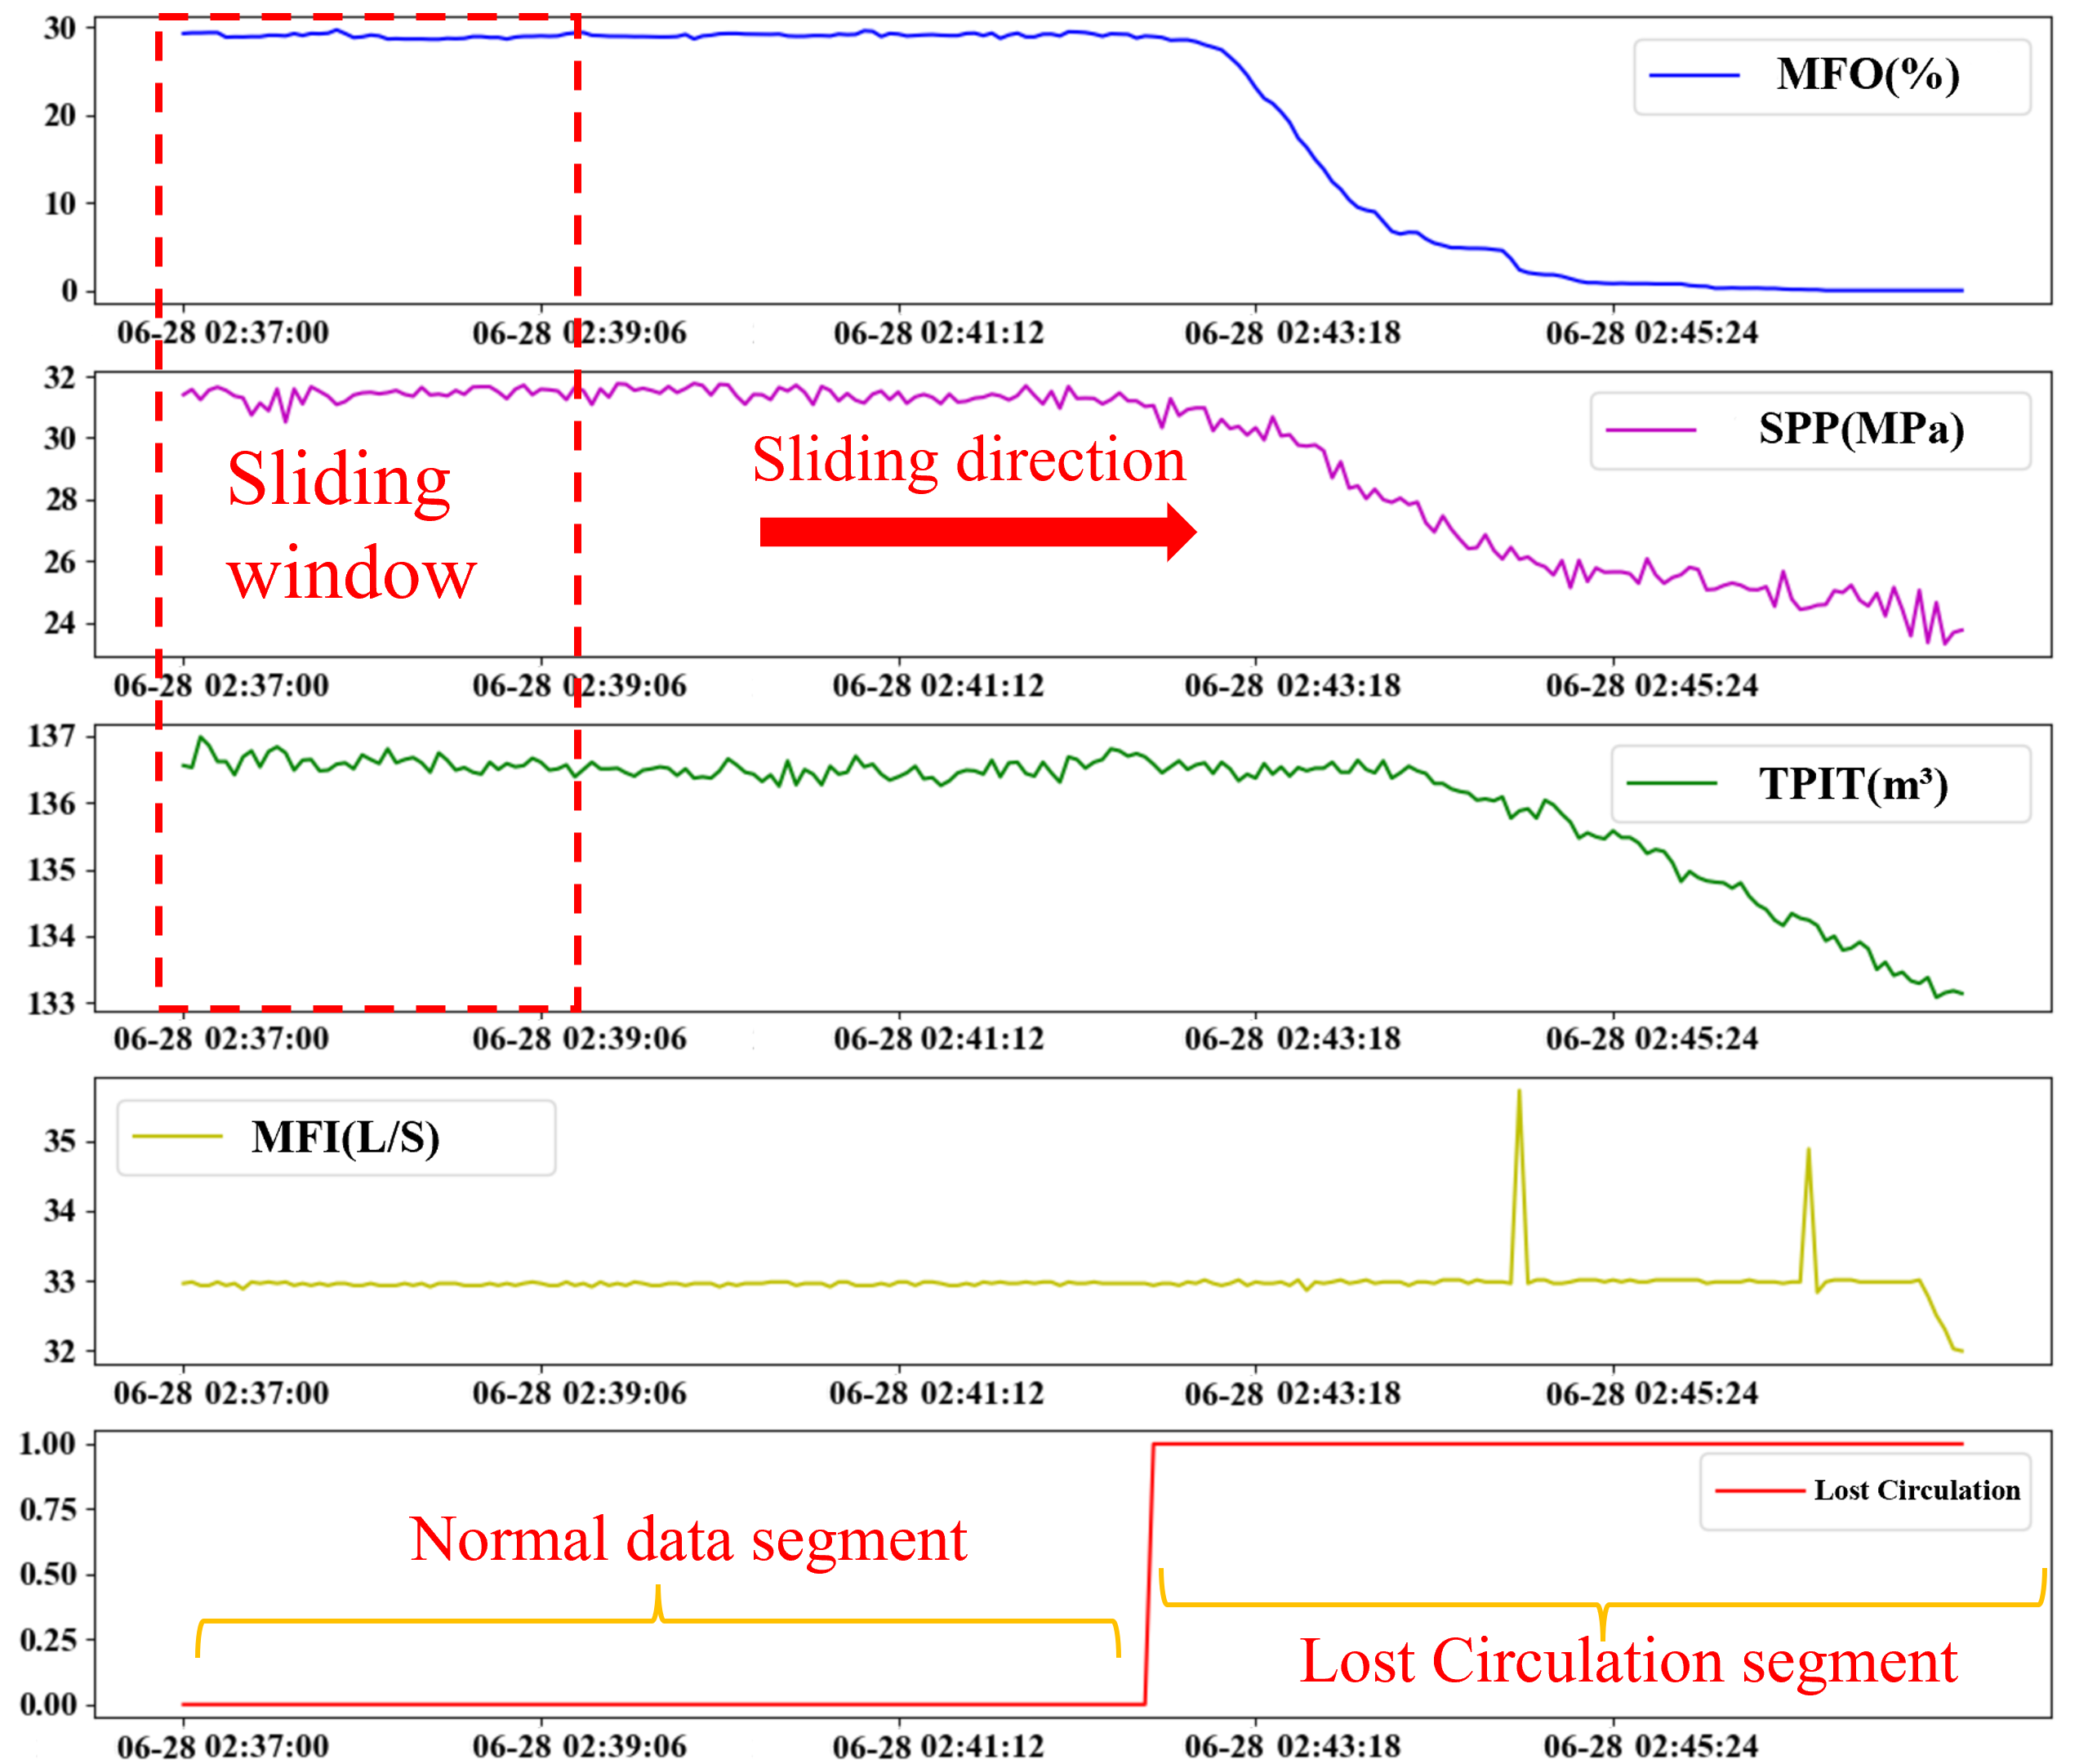
\includegraphics[width=0.75\linewidth]{图片/滑动窗口.png}
    \caption{Time series sample construction based on sliding window method}
    \label{fig:Time series sample construction based on sliding window method}
\end{figure}

%%%%%%%%%%%%%%%%%%%%%%%%%%%%%%%%%%%%%%%%%%
\subsection{Wavelet transform based temporal feature enhancement}

The key factors of the wavelet transform effect are the number of wavelet decomposition layers and the type of wavelet function, and the selection of appropriate parameters can significantly improve the transform effect. According to the characteristics of the lost circulation time series data, this study adopts Haar wavelet function to transform the original feature signal, and sets the number of decomposition layers to 5. Taking SPP as an example, the result after its reconstruction with 5 levels of decomposition is shown in Fig.  \ref{fig:Haar five-level wavelet decomposition reconstruction for SPPs}, where the low-frequency approximate features are similar to the original features, while the high-frequency detail features (d1~d5) show different degrees of oscillation characteristics.

\begin{figure}[h]
    \centering
    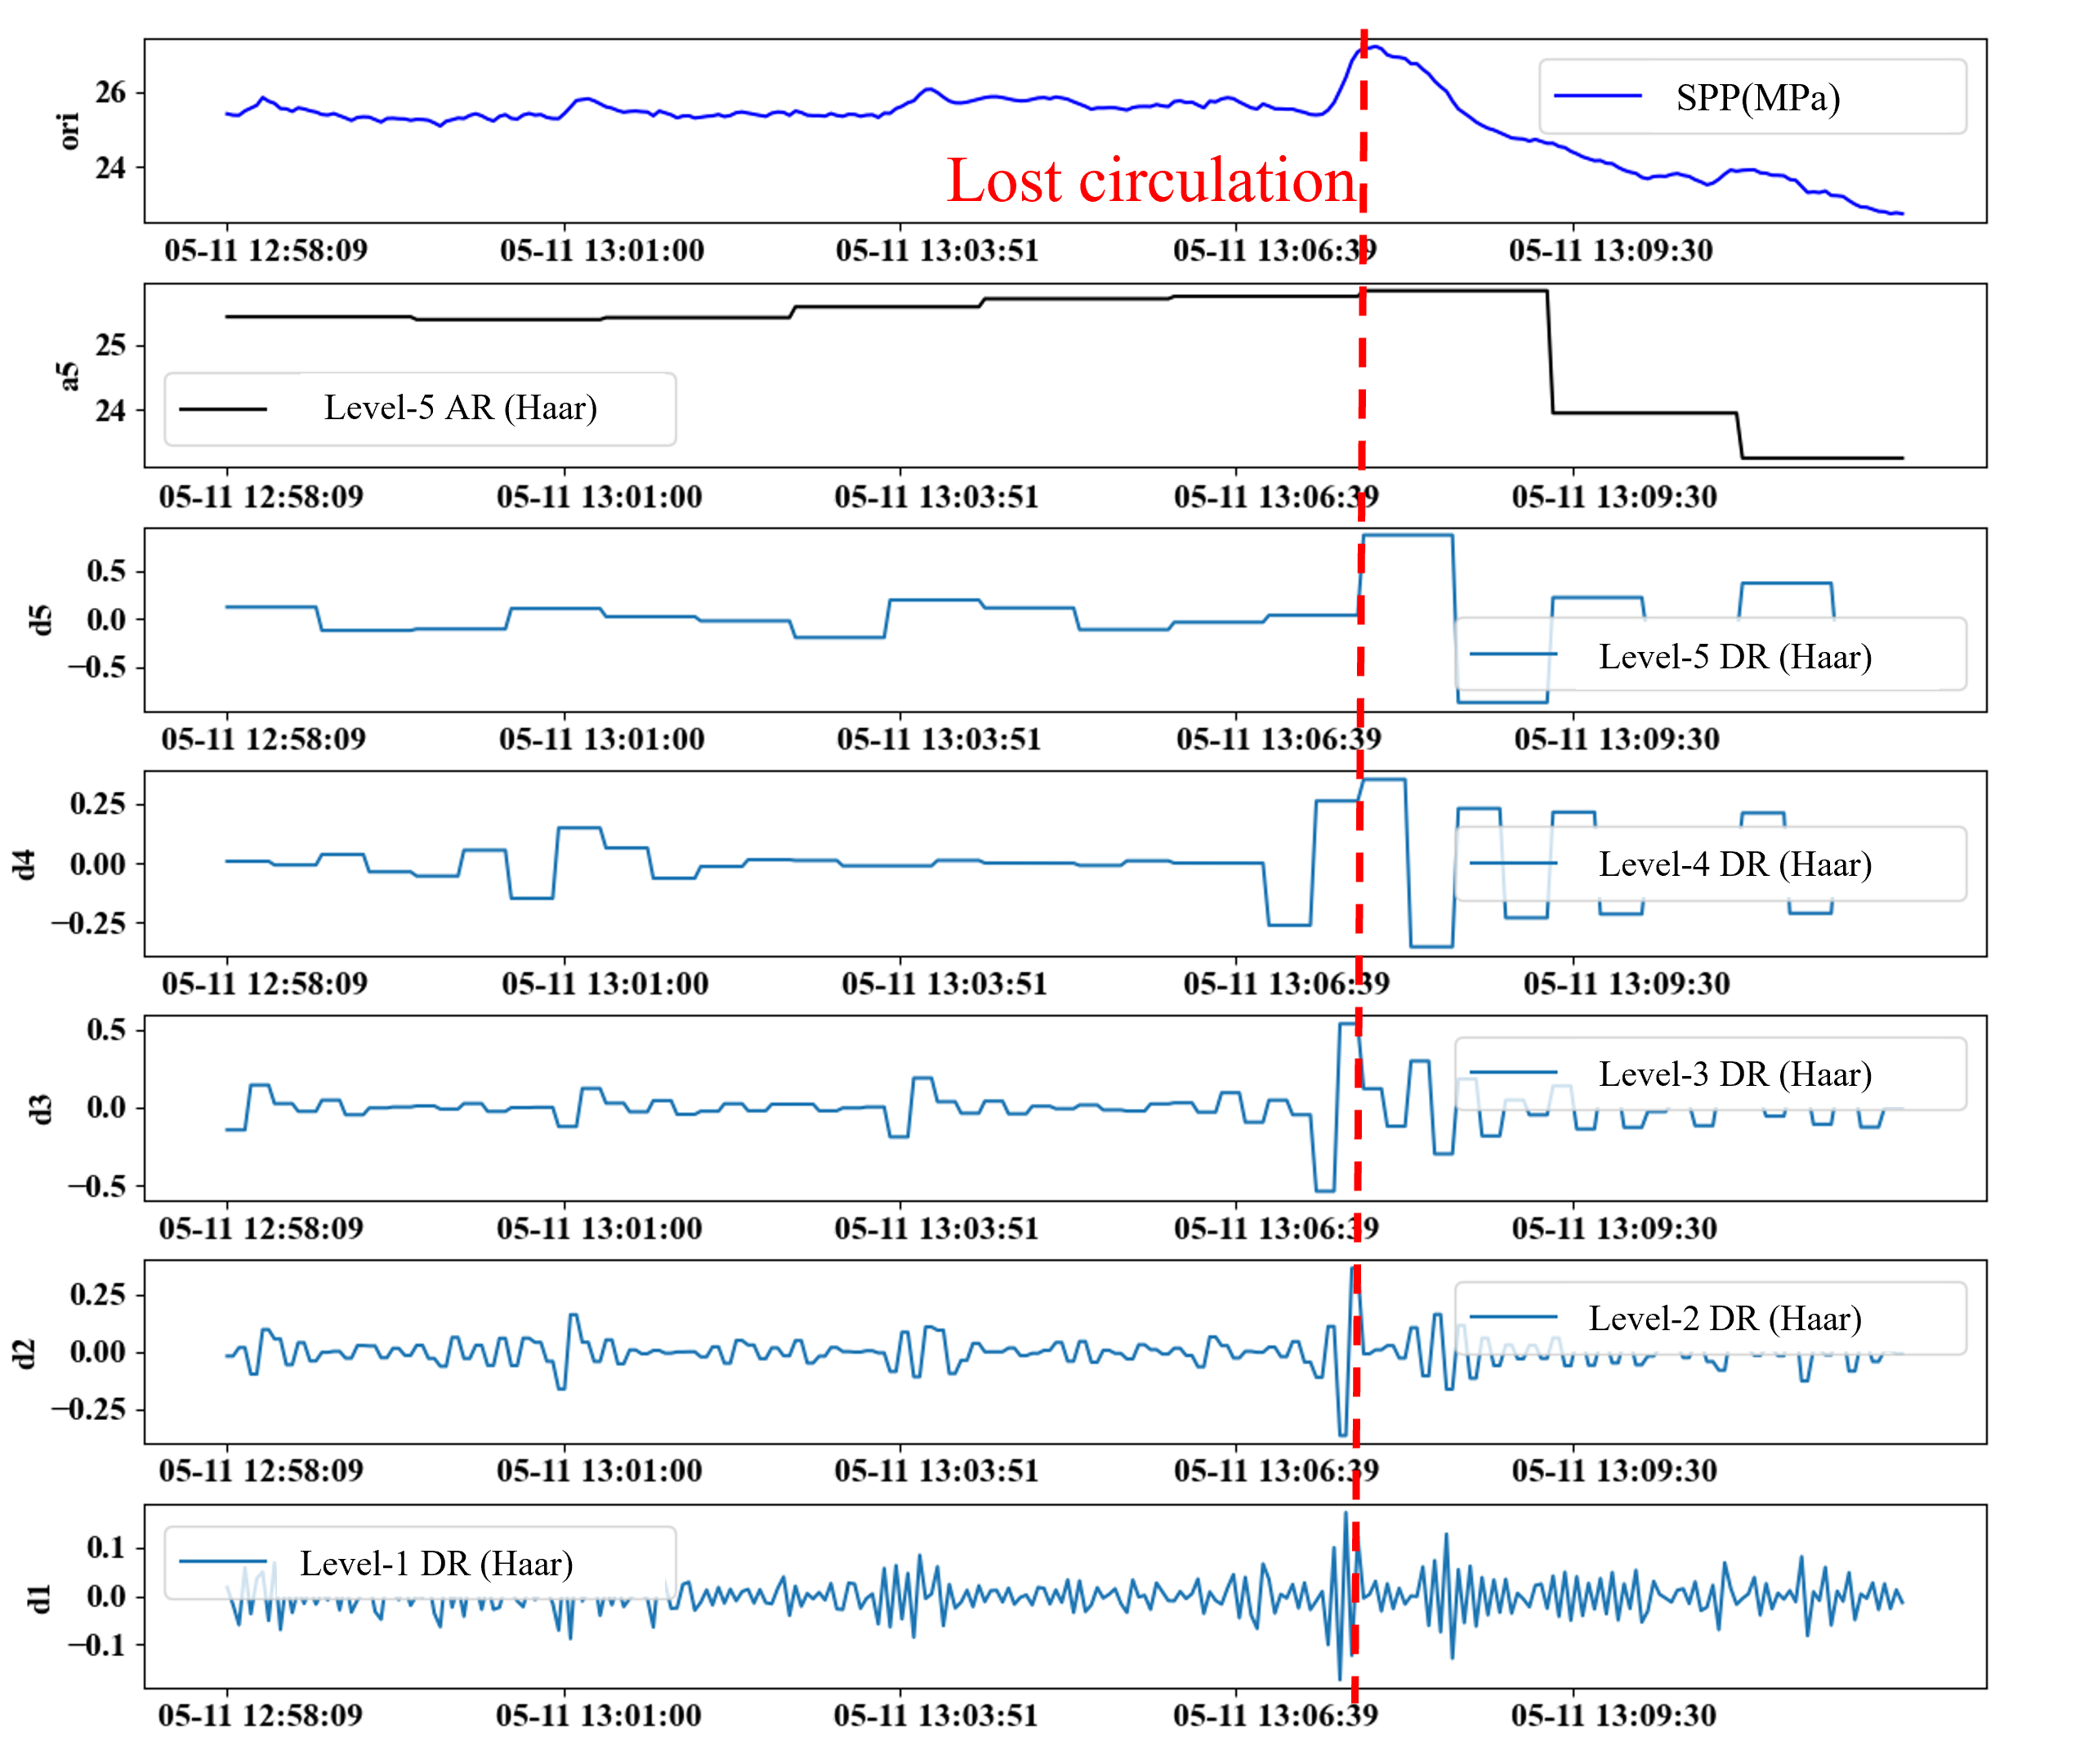
\includegraphics[width=0.75\linewidth]{图片/5级小波分解.png}
    \caption{Haar five-level wavelet decomposition reconstruction for SPPs}
    \label{fig:Haar five-level wavelet decomposition reconstruction for SPPs}
\end{figure}

Among the high-frequency detail features, the oscillation frequencies of d1 and d2 are higher but the difference is not obvious, and the oscillation patterns of d4 and d5 are too discrete to effectively describe the continuous changes before and after the lost circulation occurs. In contrast, d3 achieves a better balance between signal continuity and amplitude fluctuation characteristics, and is able to more clearly characterise the data fluctuations before and after the lost circulation. Therefore, the 3-level wavelet decomposition is the most effective.

After wavelet transforming the seven  lost circulation time series features, the correlation between the new features and the  lost circulation labels is analysed by the correlation coefficient method, and the results are shown in Figure  \label{fig:Sperman correlation coefficients of features before and after wavelet transformation}. Although the Spearman correlation coefficients of the new features have decreased, the transformed features of Hook load, SPP, TPIT and MFO are still strongly correlated with the lost circulation risk labels, and these four features are finally selected as the effective enhancement features of the lost circulation risk .

\begin{figure}[h]
    \centering
    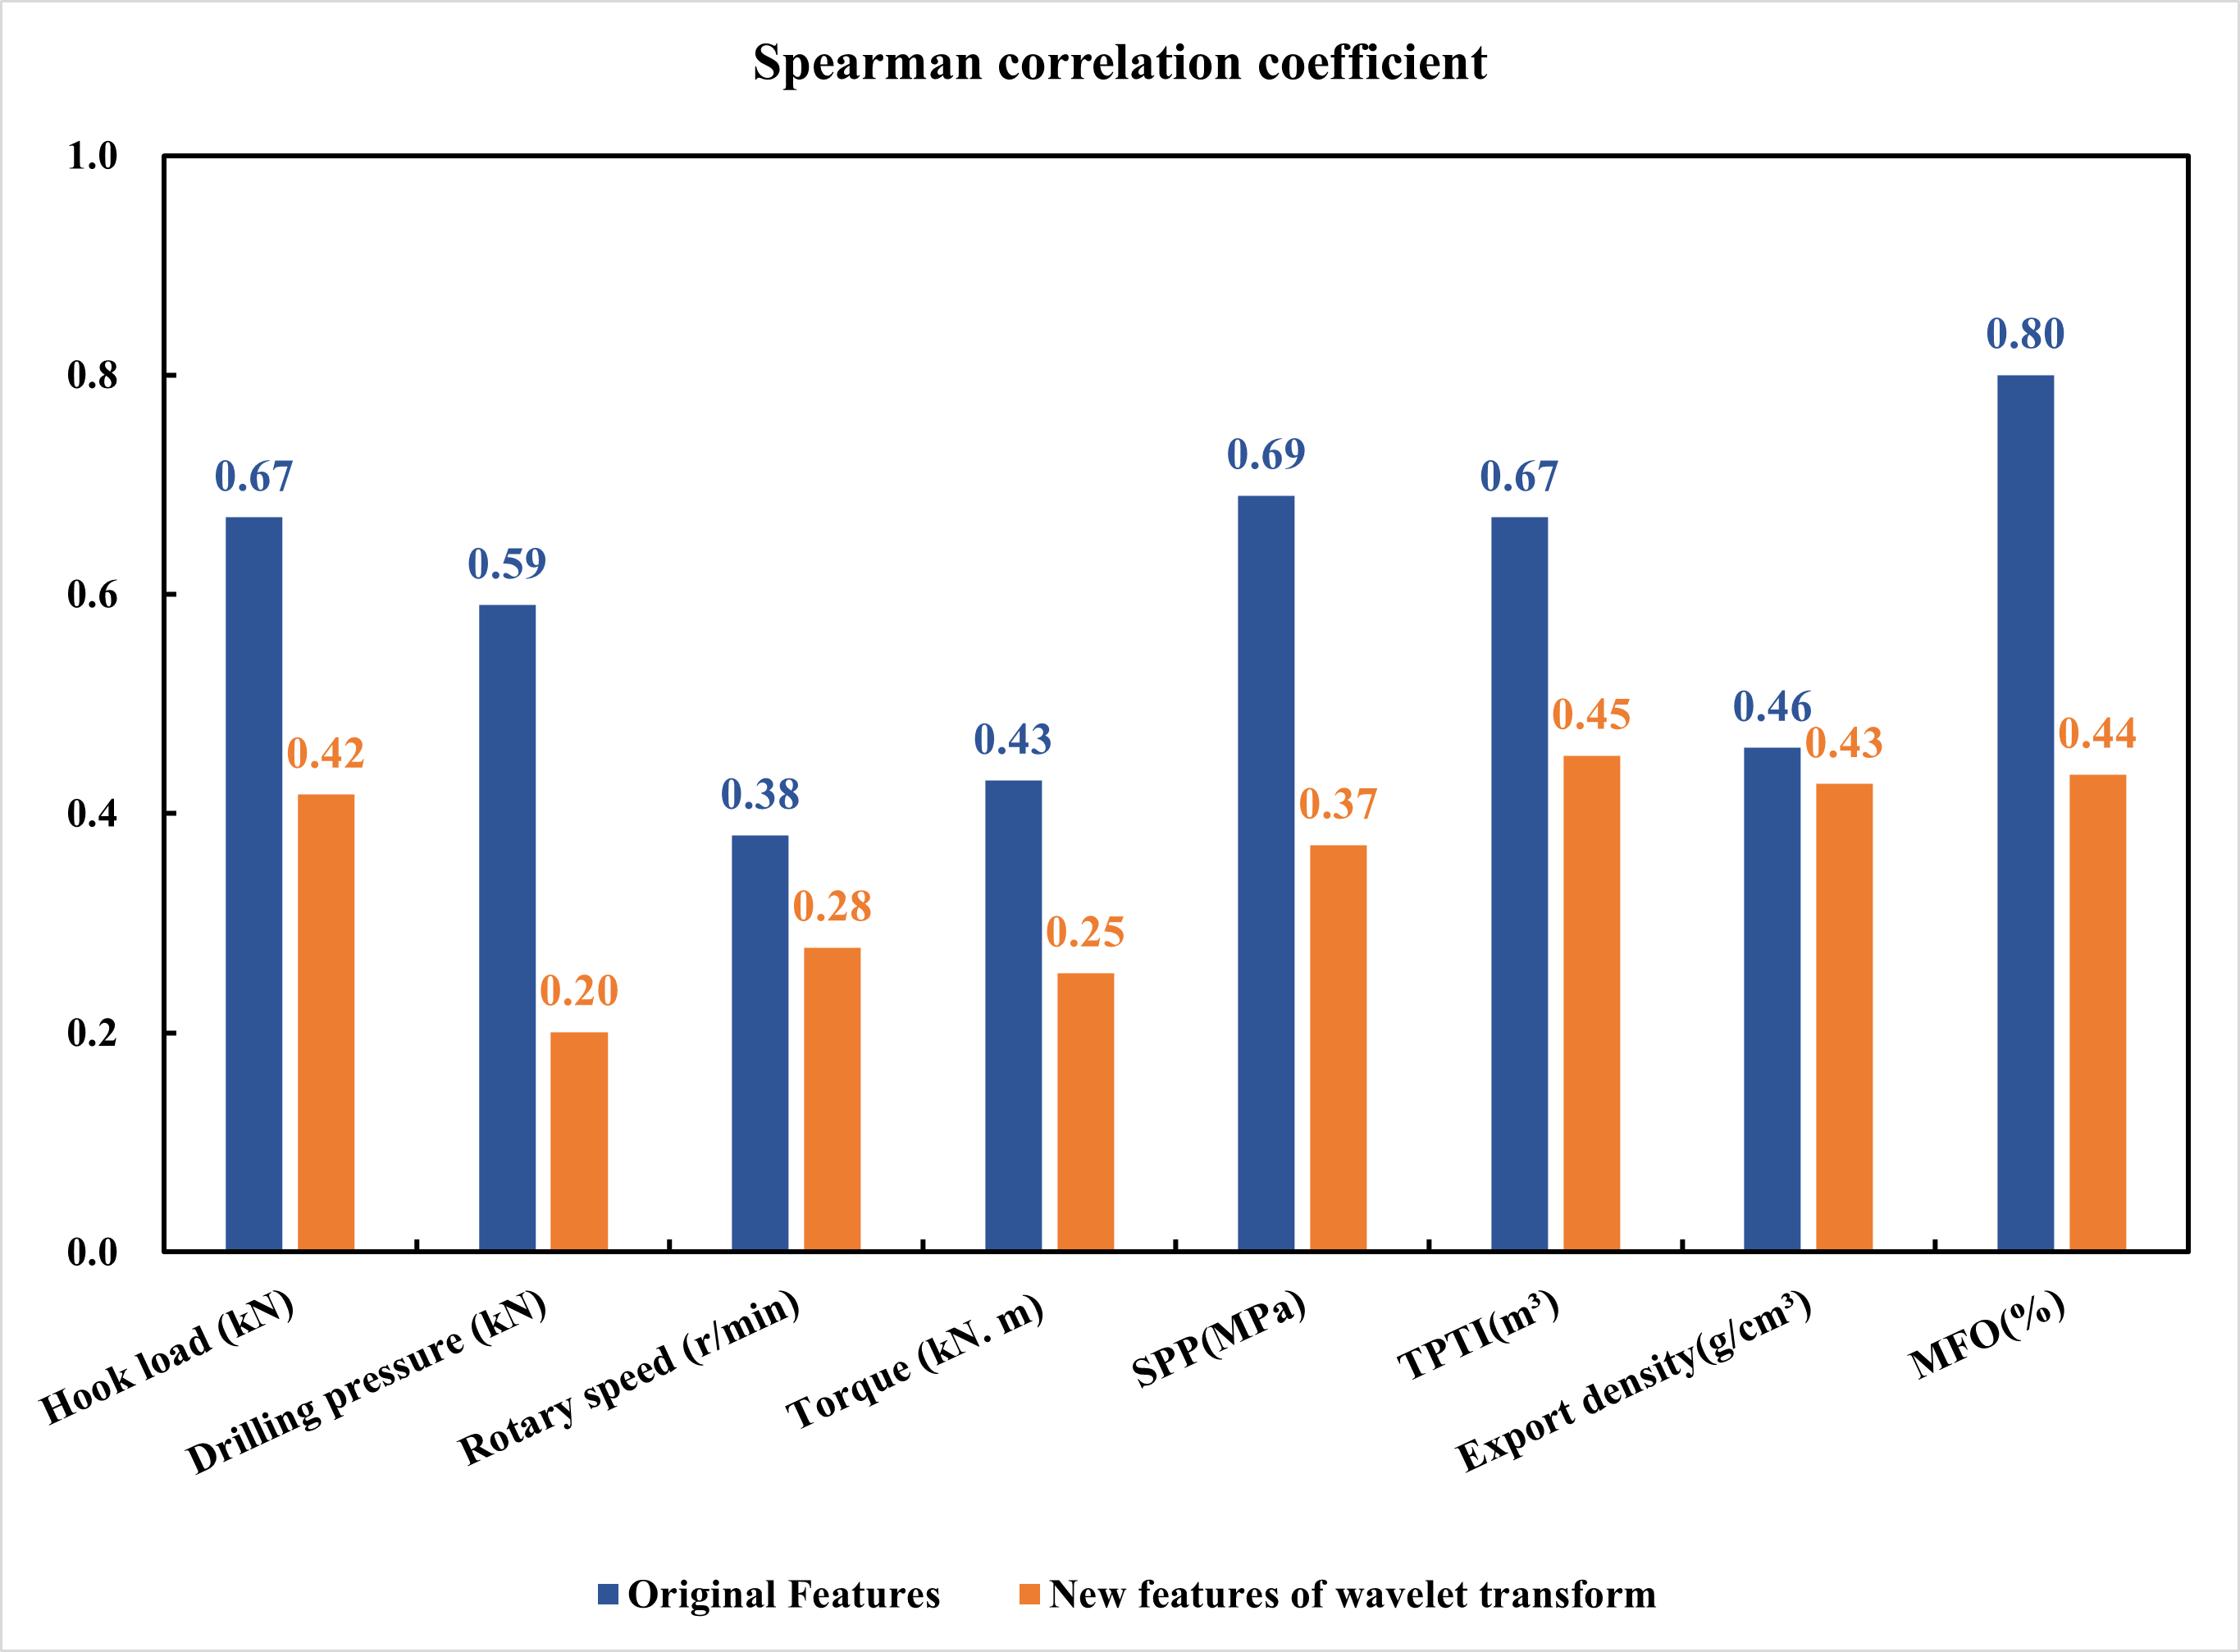
\includegraphics[width=0.75\linewidth]{图片/spearman相关系数.png}
    \caption{Spearman correlation coefficients of features before and after wavelet transformation}
    \label{fig:Spearman correlation coefficients of features before and after wavelet transformation}
\end{figure}
%%%%%%%%%%%%%%%%%%%%%%%%%%%%%%%%%%%%%%%%%%
\subsection{TimeGAN-based temporal data expansion}

In order to ascertain the efficacy of the TimeGAN model in the generation of lost circulation time-series data, this study utilises a training set comprising over 4,700 lost circulation time-series data points from the previously constructed lost circulation recording time-series dataset. In order to meet the input format requirements of the TimeGAN model, the lost circulation time-series data are initially constructed into fixed-window time-series samples using the sliding-window method and subsequently normalised. 

The TimeGAN network constructed in this study generated the lost circulation time series data after 20,000 iterations. The comparison of the generated results with the real samples is shown in Figure   \label{fig:TimeGAN Generation of Lost Circulation Time Series Data}, where the horizontal axis is the time step and the vertical axis is the normalised values of the feature parameters. While the generated data are numerically distinct from the actual data, they exhibit a certain degree of time series correlation. 

\begin{figure}[h]
    \centering
    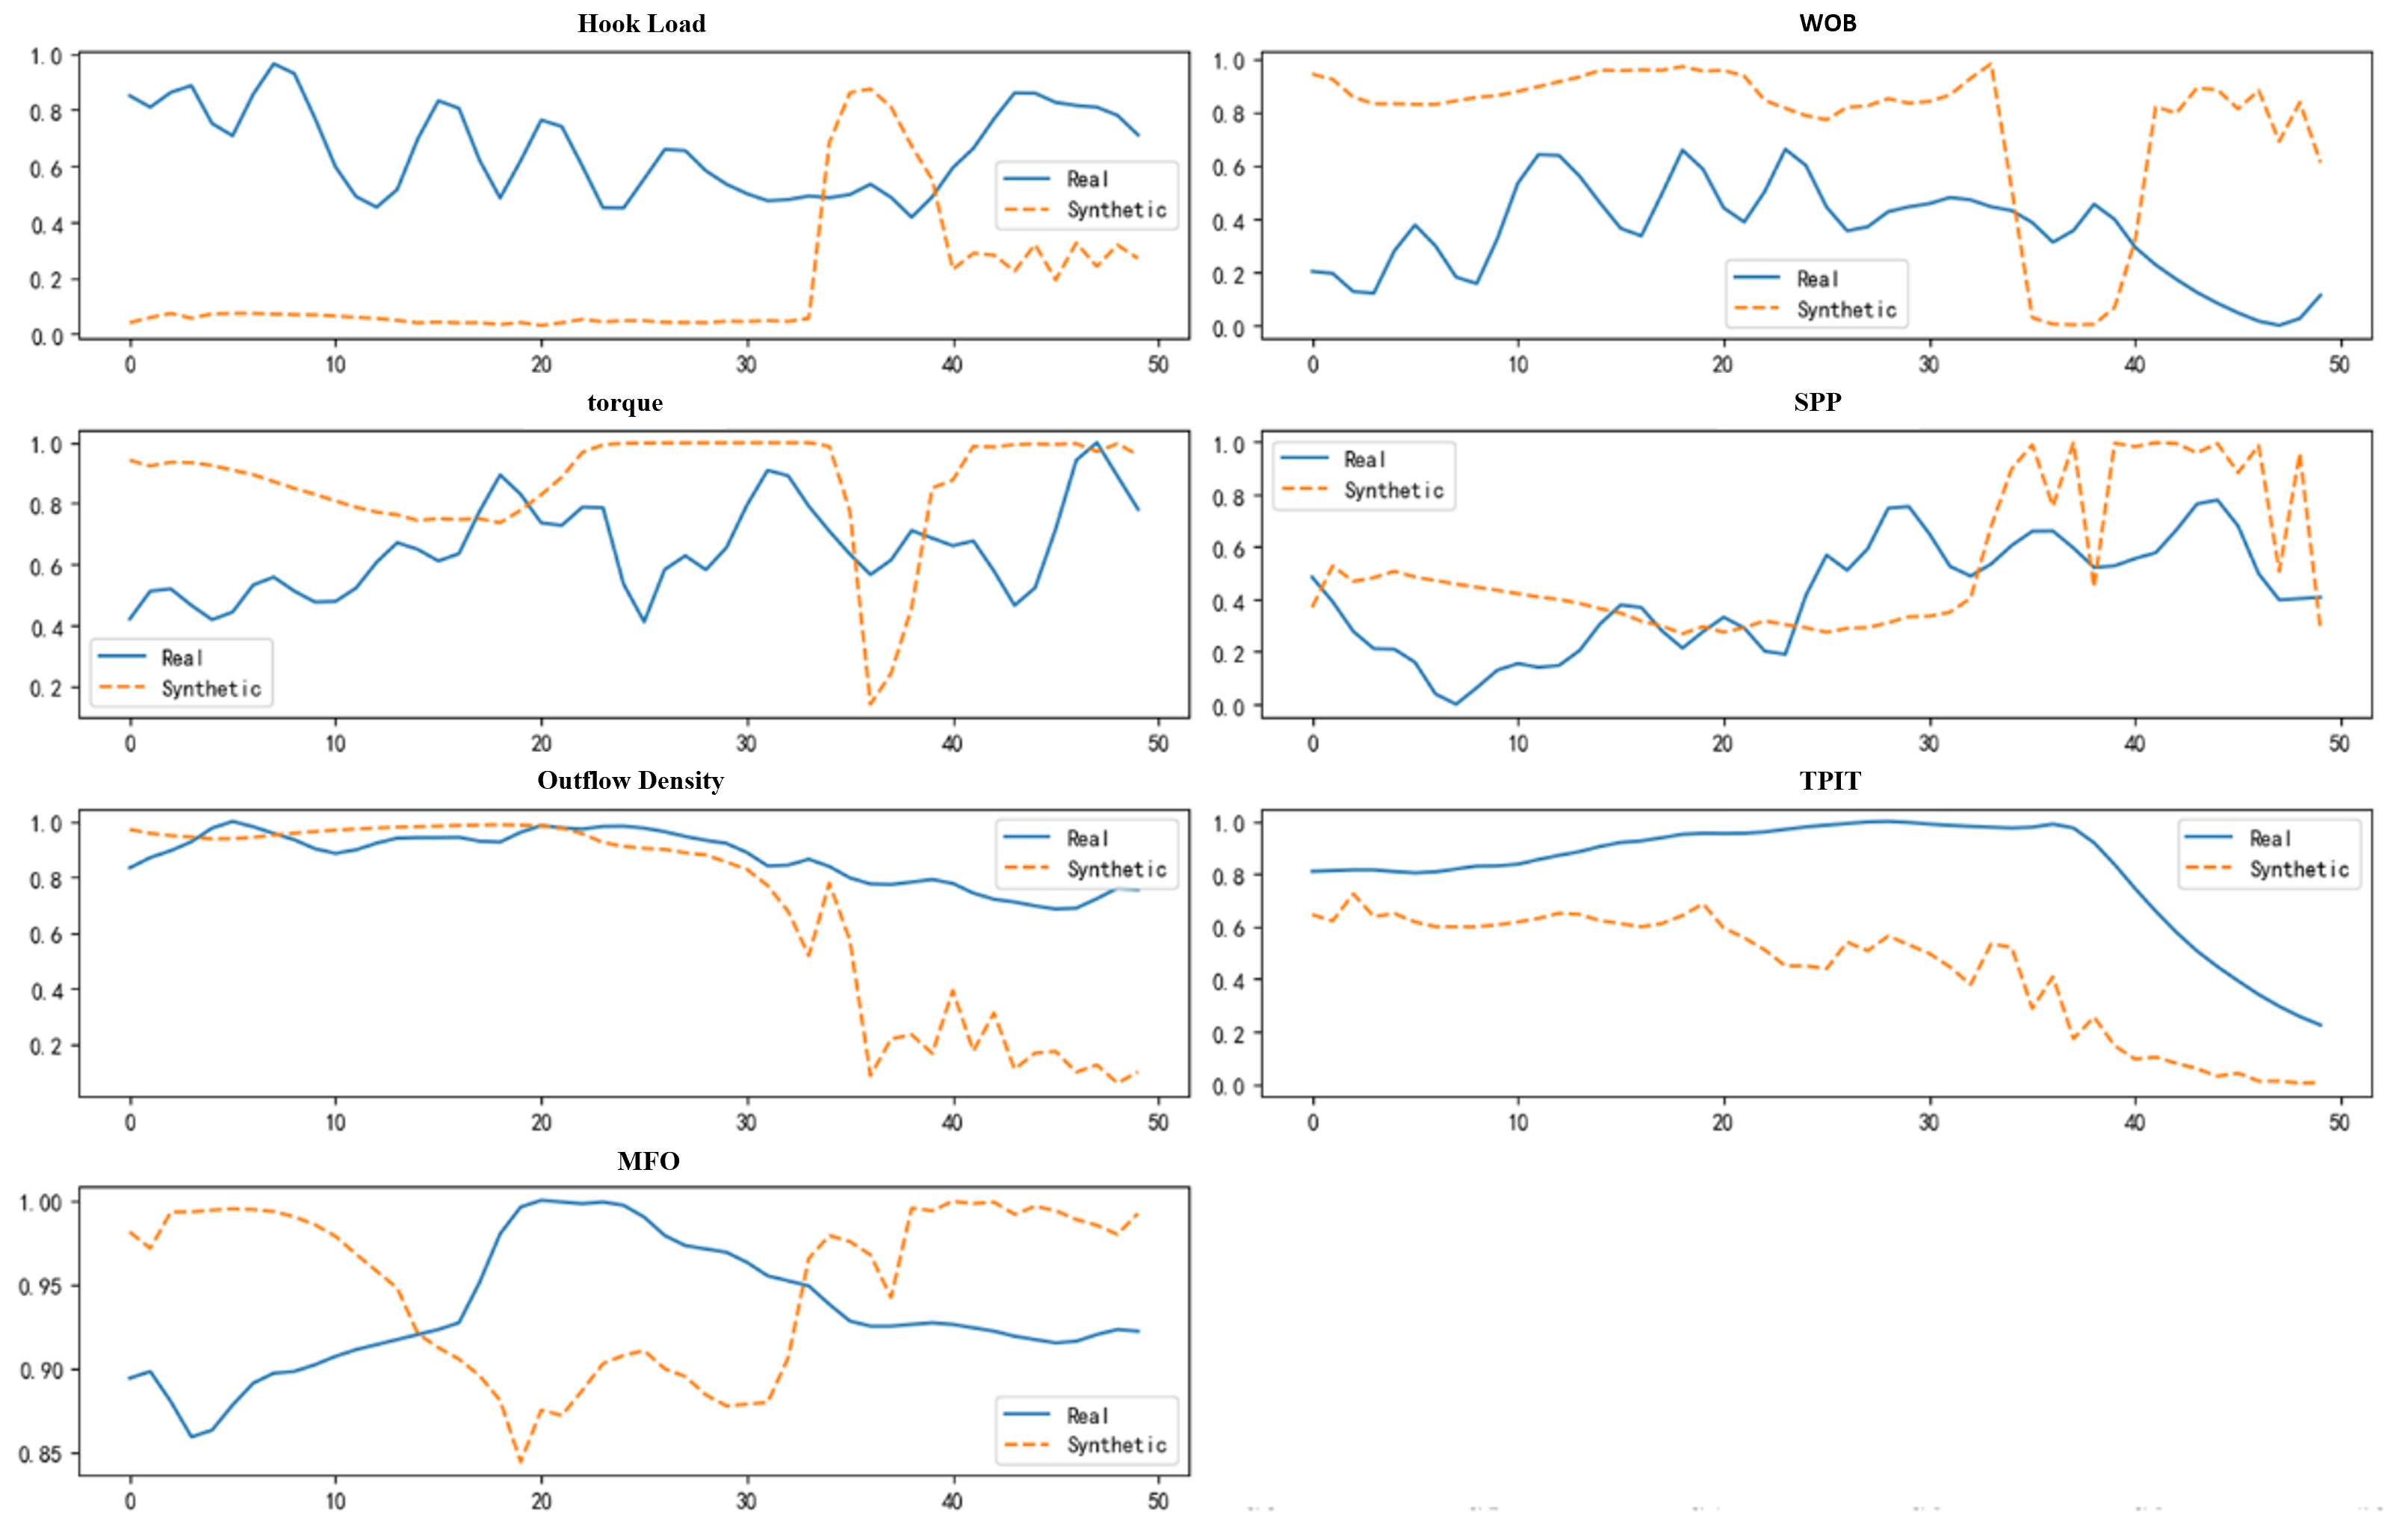
\includegraphics[width=0.75\linewidth]{图片/timeGan数据生成.png}
    \caption{TimeGAN Generation of Lost Circulation Time Series Data}
    \label{fig:TimeGAN Generation of Lost Circulation Time Series Data}
\end{figure}


The results subsequent to PCA and t-SNE dimensionality reduction are demonstrated in Figure \label{fig:PCA and TSNE visualisation results of generated data versus raw data}. The proximity of the generated data (red dots) to the original data (black dots) indicates a resemblance between the static and temporal characteristics of the generated data and the real data. As demonstrated in the figure, irrespective of the dimensionality reduction outcomes of PCA or t-SNE, the generated data are distributed in proximity to the hotspot region of the original data and are equally sparse in the sparse region of the original data. This suggests that the TimeGAN-generated lost circulation temporal data features are more aligned with the real data.

\begin{figure}[h]
    \centering
    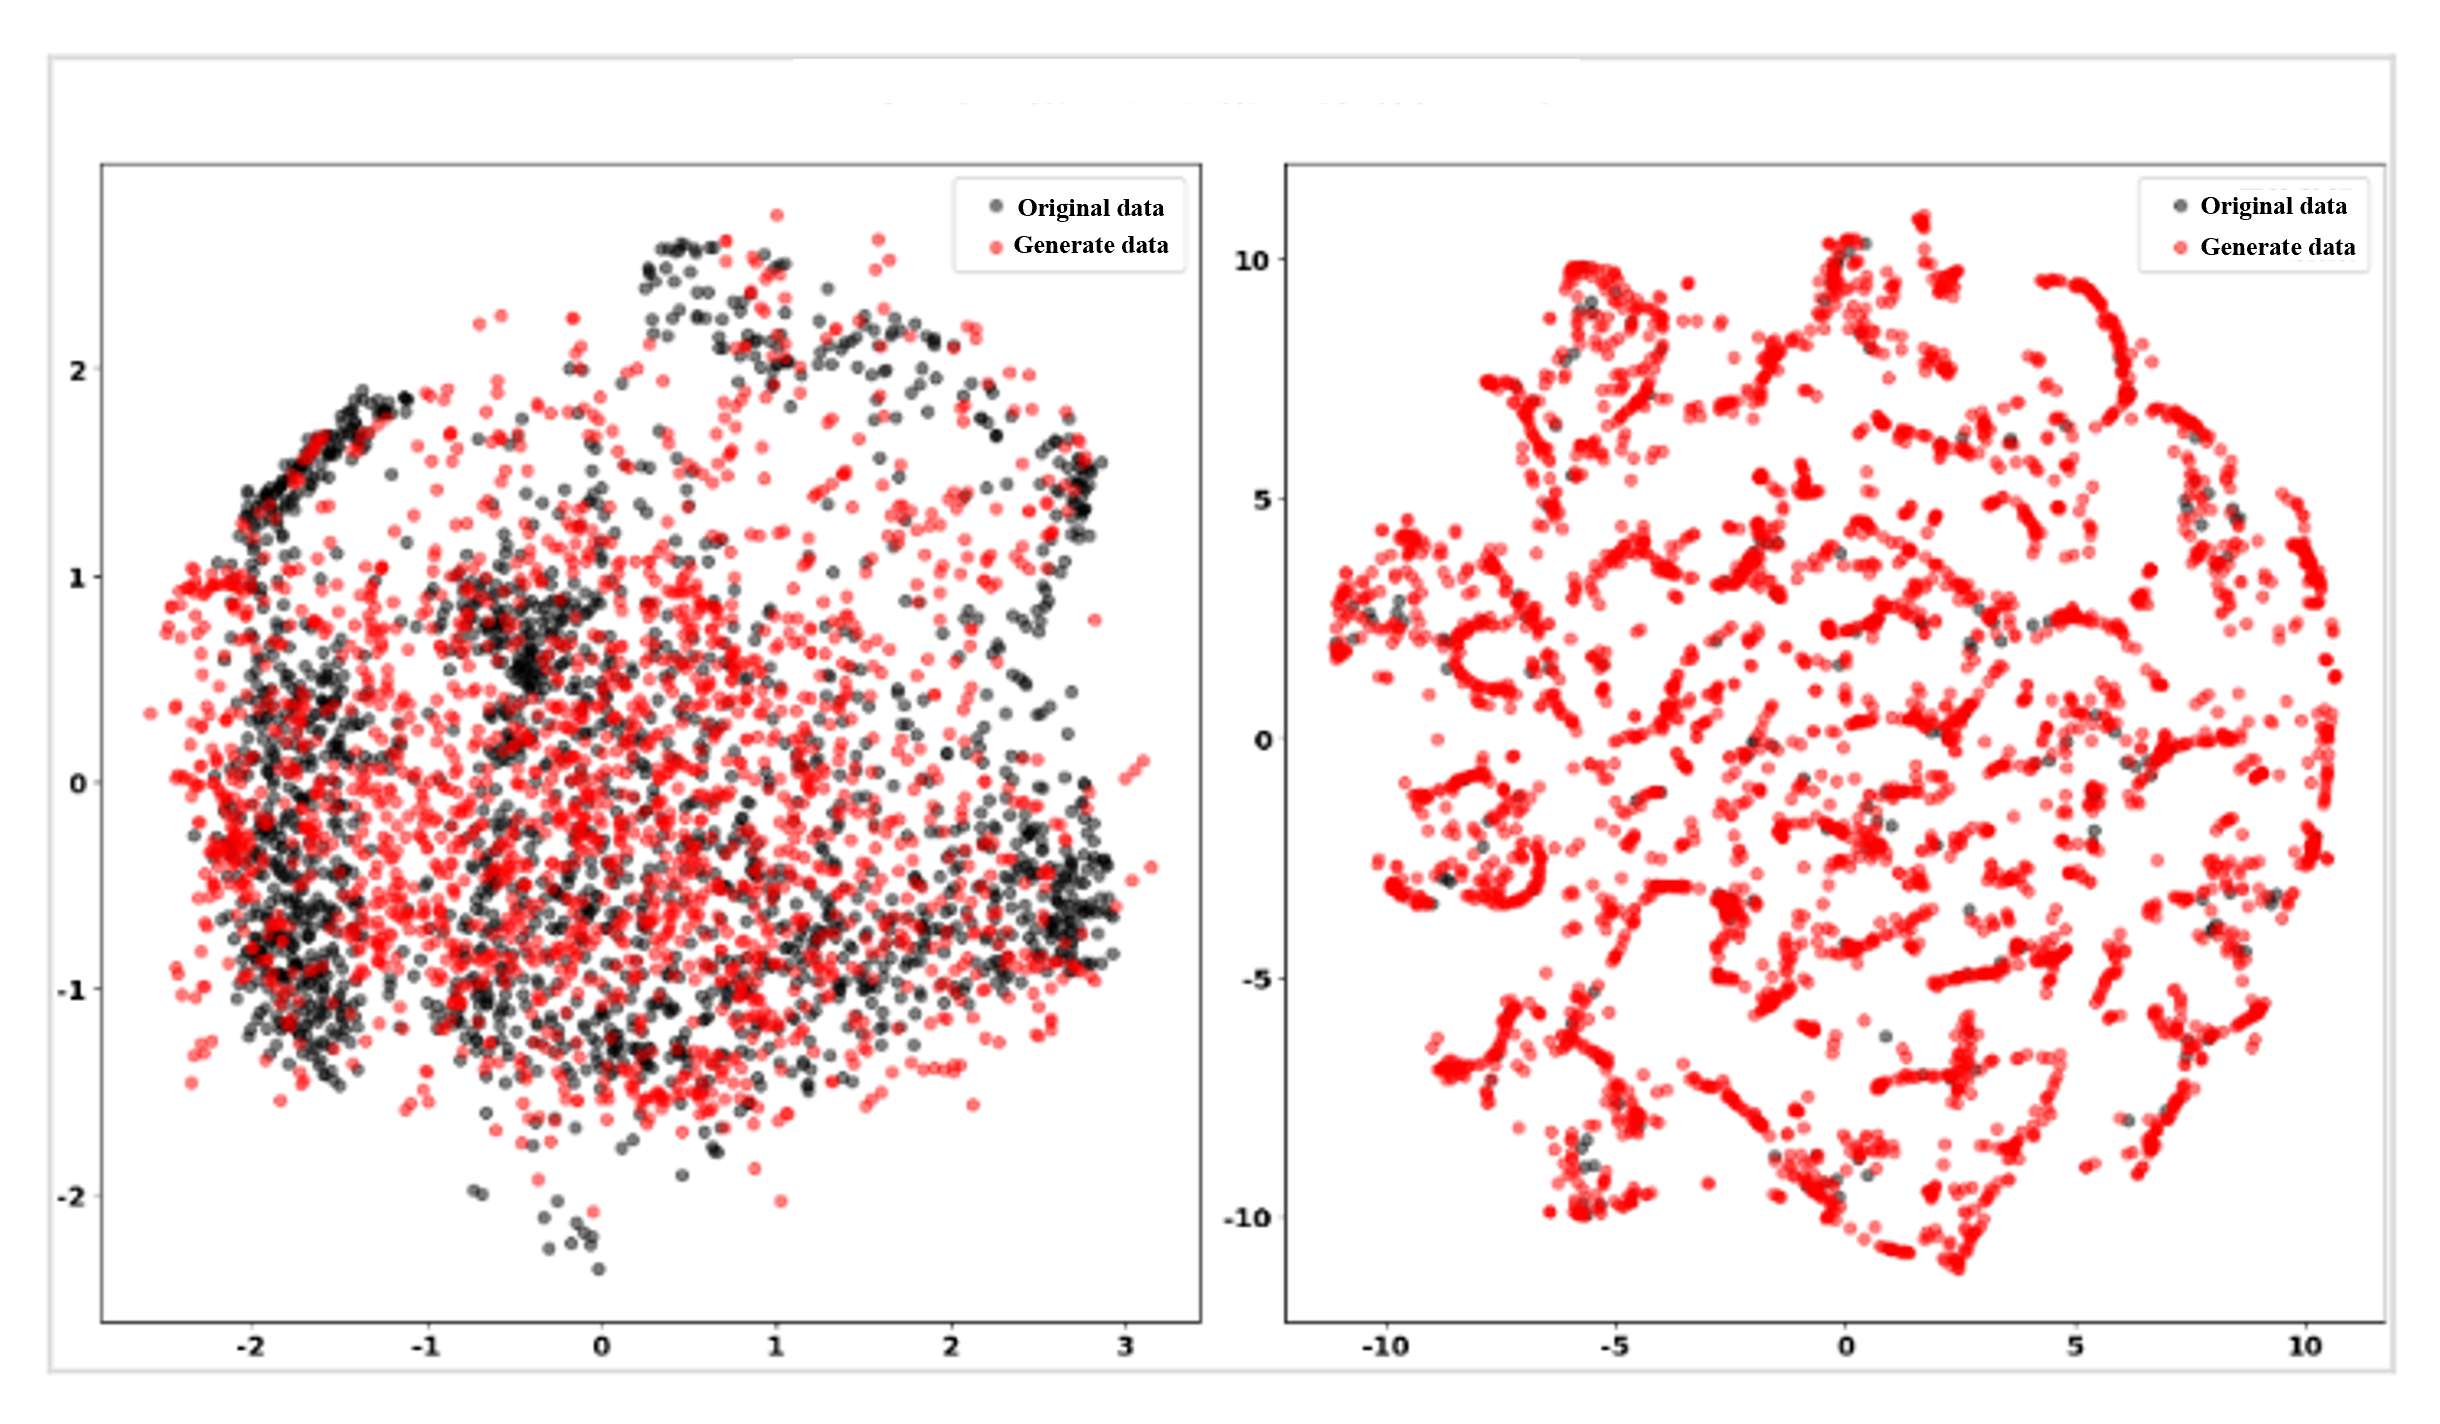
\includegraphics[width=0.75\linewidth]{图片/pca tsne.png}
    \caption{PCA and TSNE visualisation results of generated data versus raw data}
    \label{fig:PCA and TSNE visualisation results of generated data versus raw data}
\end{figure}



%%%%%%%%%%%%%%%%%%%%%%%%%%%%%%%%%%%%%%%%%%
\section{Model Construction}
\subsection{Evaluation metrics}

A significant aspect of employing machine learning methodologies to address engineering challenges is the assessment of algorithmic models' efficacy. this study employs four evaluation metrics (i.e. Accuracy, Recall, Missing Alarm and False Alarm\cite{SunW2023}) to evaluate the performance of diverse models in identifying lost circulation risk \cite{ZZY2024}. The calculation formulae for each evaluation index are delineated in Table 1 and the subsequent equation.

\begin{table}[h]
\centering
\begin{tabular}{lcc}
\hline
                      & \textbf{Positive Class} & \textbf{Negative Class} \\ \hline
\textbf{Positive Class} & TP                      & FN                      \\
\textbf{Negative Class} & FP                      & TN                      \\ \hline
\end{tabular}
\caption{True Result vs. Forecast Result}
\label{True Result vs. Forecast Result}
\end{table}
TP is defined as the number of samples that are correctly classified as positive by the model;
FN is defined as the number of samples that are incorrectly classified as negative by the model;
FP is defined as the number of samples that are incorrectly classified as positive by the model; and
TN is defined as the number of samples that are correctly classified as negative by the model.

$$ A c c u r a c y = \frac { T P + T N } { T P + F N + T N + F P }\quad (10)$$
$$ R e c a l l = \frac { T P } { T P + F N } \quad (11)$$

$$ M i s sin g A l a r m = \frac { F N } { T P + F N } \quad (12)$$

$$ F a l s e A l a r m = \frac { F P } { T P + F P } \quad (13)$$

In a classification model, \textbf{accuracy} represents the proportion of correctly classified samples to the total number of samples. \textbf{Recall}, specifically for positive cases, is the proportion of true positive samples correctly identified out of all actual positive samples. \textbf{Missing Alarm} refers to the fraction of actual lost circulation samples that are incorrectly classified as non-lost circulation, representing missed detections. Conversely, \textbf{False Alarm} denotes the fraction of non-lost circulation samples that are incorrectly classified as lost circulation, indicating misclassifications among predicted positive samples.

%%%%%%%%%%%%%%%%%%%%%%%%%%%%%%%%%%%%%%%%%%
\subsection{Parameter setting }

In order to ascertain the efficacy of the TimeGAN model in the generation of lost circulation time-series data, this study utilises a dataset comprising over 4,700 instances of lost circulation time-series data, as previously constructed from the time-series dataset of lost circulation recordings. In order to satisfy the input requirements of the TimeGAN model, the well-loss time-series data are initially configured as time-series samples with fixed window intervals, employing the sliding window method and normalised.

\subsection{Hyper-parameter optimisation}

In the context of training a model of this nature, there are two primary types of hyperparameter that demand attention: training hyperparameters and structural hyperparameters. The former primarily govern the model's training process, while the latter determine its structural design. 

Given the vast number of hyperparameters and the wide range of values they can assume, this study employs the open-source library Optuna for the optimisation of hyperparameters. This library is a specialised open-source toolkit developed for the optimisation of hyperparameters in deep learning models. It is capable of automatically searching for the optimal hyperparameter configurations within the hyperparameter space by using Bayesian optimisation and genetic algorithms, among other methods. It is notable for its simplicity and ease of use, coupled with a high degree of flexibility, and its compatibility with mainstream deep learning models such as PyTorch and TensorFlow, TensorFlow, and other mainstream deep learning platforms.

In the experiment, the native TimeGAN network in the ydata-synthetic library based on the Python language is utilised to construct the data expansion generation model, and the primary parameter settings of the model are exhibited in Table \label{TimeGAN parameter settings}.

\begin{table}[h]
\centering
\begin{tabular}{lll}
\toprule
\textbf{Parameter Name} & \textbf{Parameter Description} & \textbf{Parameter Setting} \\ 
\midrule
\textbf{Seq\_len}       & Sample time window length      & 50                          \\ 
\textbf{N\_seq}         & Data feature dimension         & 7                           \\ 
\textbf{Hidden\_dim}    & Generator hidden layer size    & 24                          \\ 
\textbf{Gamma}          & Discriminator loss weight      & 1                           \\ 
\textbf{Noise\_dim}     & Generator noise dimension      & 32                          \\ 
\textbf{Batch\_size}    & Training batch size            & 128                         \\ 
\textbf{Learning\_rate} & Learning rate                  & 0.001                       \\ 
\bottomrule
\end{tabular}
\caption{TimeGAN parameter settings}
\label{TimeGAN parameter settings}
\end{table}

\subsection{Hybrid Loss Function Design }
 
In order to enhance the performance of the lost circulation detection model, a hybrid loss function is designed in this study to combine multiple loss objectives to balance the prediction accuracy and feature selection capability, while effectively suppressing the overfitting phenomenon. The hybrid loss function consists of the mean square error (MSE) of coordinate regression and the cross-entropy loss of confidence to balance the demands of the classification task and the regression task. The hybrid loss function expression is:
$$ L _ { t o t a l } = \lambda _ { 1 } L _ { M S E } + \lambda _ { 2 } L _ { C E } + \lambda _ { 3 } L _ { r e g }\quad (14)$$

\( L _ { M S E } \): The Mean Squared Error (MSE) loss, which is used to measure the accuracy of the lost circulation feature regression task, is given by:
$$ L _ { M S E } = \frac { 1 } { N } \sum _ { i = 1 } ^ { N } ( y _ { i } - \widehat { y } _ { i } ) ^ { 2 }\quad (15)$$

The true value is denoted by \({ y } _ { i } \), the model prediction by \(\widehat { y } _ { i }\) , and the number of samples by \(N\).


\(L _ { CE}\): Cross Entropy Loss, which is employed to evaluate the confidence of the occurrence of lost circulation in the classification task, is given by:
\[{{L}_{CE}}=-\frac{1}{N}\underset{i=1}{\overset{N}{\mathop \sum }}\,\left[ {{y}_{i}}\log {{{\hat{y}}}_{i}}+(1-{{y}_{i}})\log (1-{{{\hat{y}}}_{i}}) \right]\quad (16)\]

Where, \({y}_{i}\) denotes the true label, and \({\hat{y}}_{i}\) denotes the probability value predicted by the model.

\({L}_{reg
}\): Regularisation Loss, which is employed to constrain the complexity of the model and enhance the feature selection capability, is given by: In this study, L1 regularisation is employed, and its formula is:
$$ L _ { r e g } = | | w | | _ { 1 } = \sum _ { j = 1 } ^ { d } | w _ { j } |\quad (17)$$

\(w\), The weight vector of the model, \(d\), is the dimension of the model parameters.

\({{\lambda }_{1}}\) ,\({{\lambda }_{2}}\) , \({{\lambda }_{3}}\):hyperparameters, which are used to regulate the importance of each loss term. 

In this study, we set \({{\lambda }_{1}}\)=0.5, \({{\lambda }_{2}}\)=0.4, \({{\lambda }_{3}}\)=0.1 to balance the prediction accuracy and feature sparsity.

%%%%%%%%%%%%%%%%%%%%%%%%%%%%%%%%%%%%%%%%%%
\section{Results and Discussion}

In this section, the analysis of the optimisation effect of different feature enhancement methods on the model is conducted, as well as the analysis of the optimisation effect of data expansion methods on the model. In addition, the analysis of the optimisation effect of feature enhancement combined with data expansion on the model is undertaken.

\subsection{Feature enhancement effect analysis}

As demonstrated in Figure \label{fig:Evaluation of feature enhancement effects}, following the implementation of wavelet transform for the purpose of feature enhancement, the evaluation indexes of the model on the test set are optimised in comparison with those prior to feature enhancement. The accuracy rate is increased by 1.2\%, the precision rate by 0.4\%, the recall rate by 2.4\%, and the leakage rate and the false alarm rate are decreased by 2.4\% and 0.4\%, respectively.

\begin{figure}[h]
    \centering
    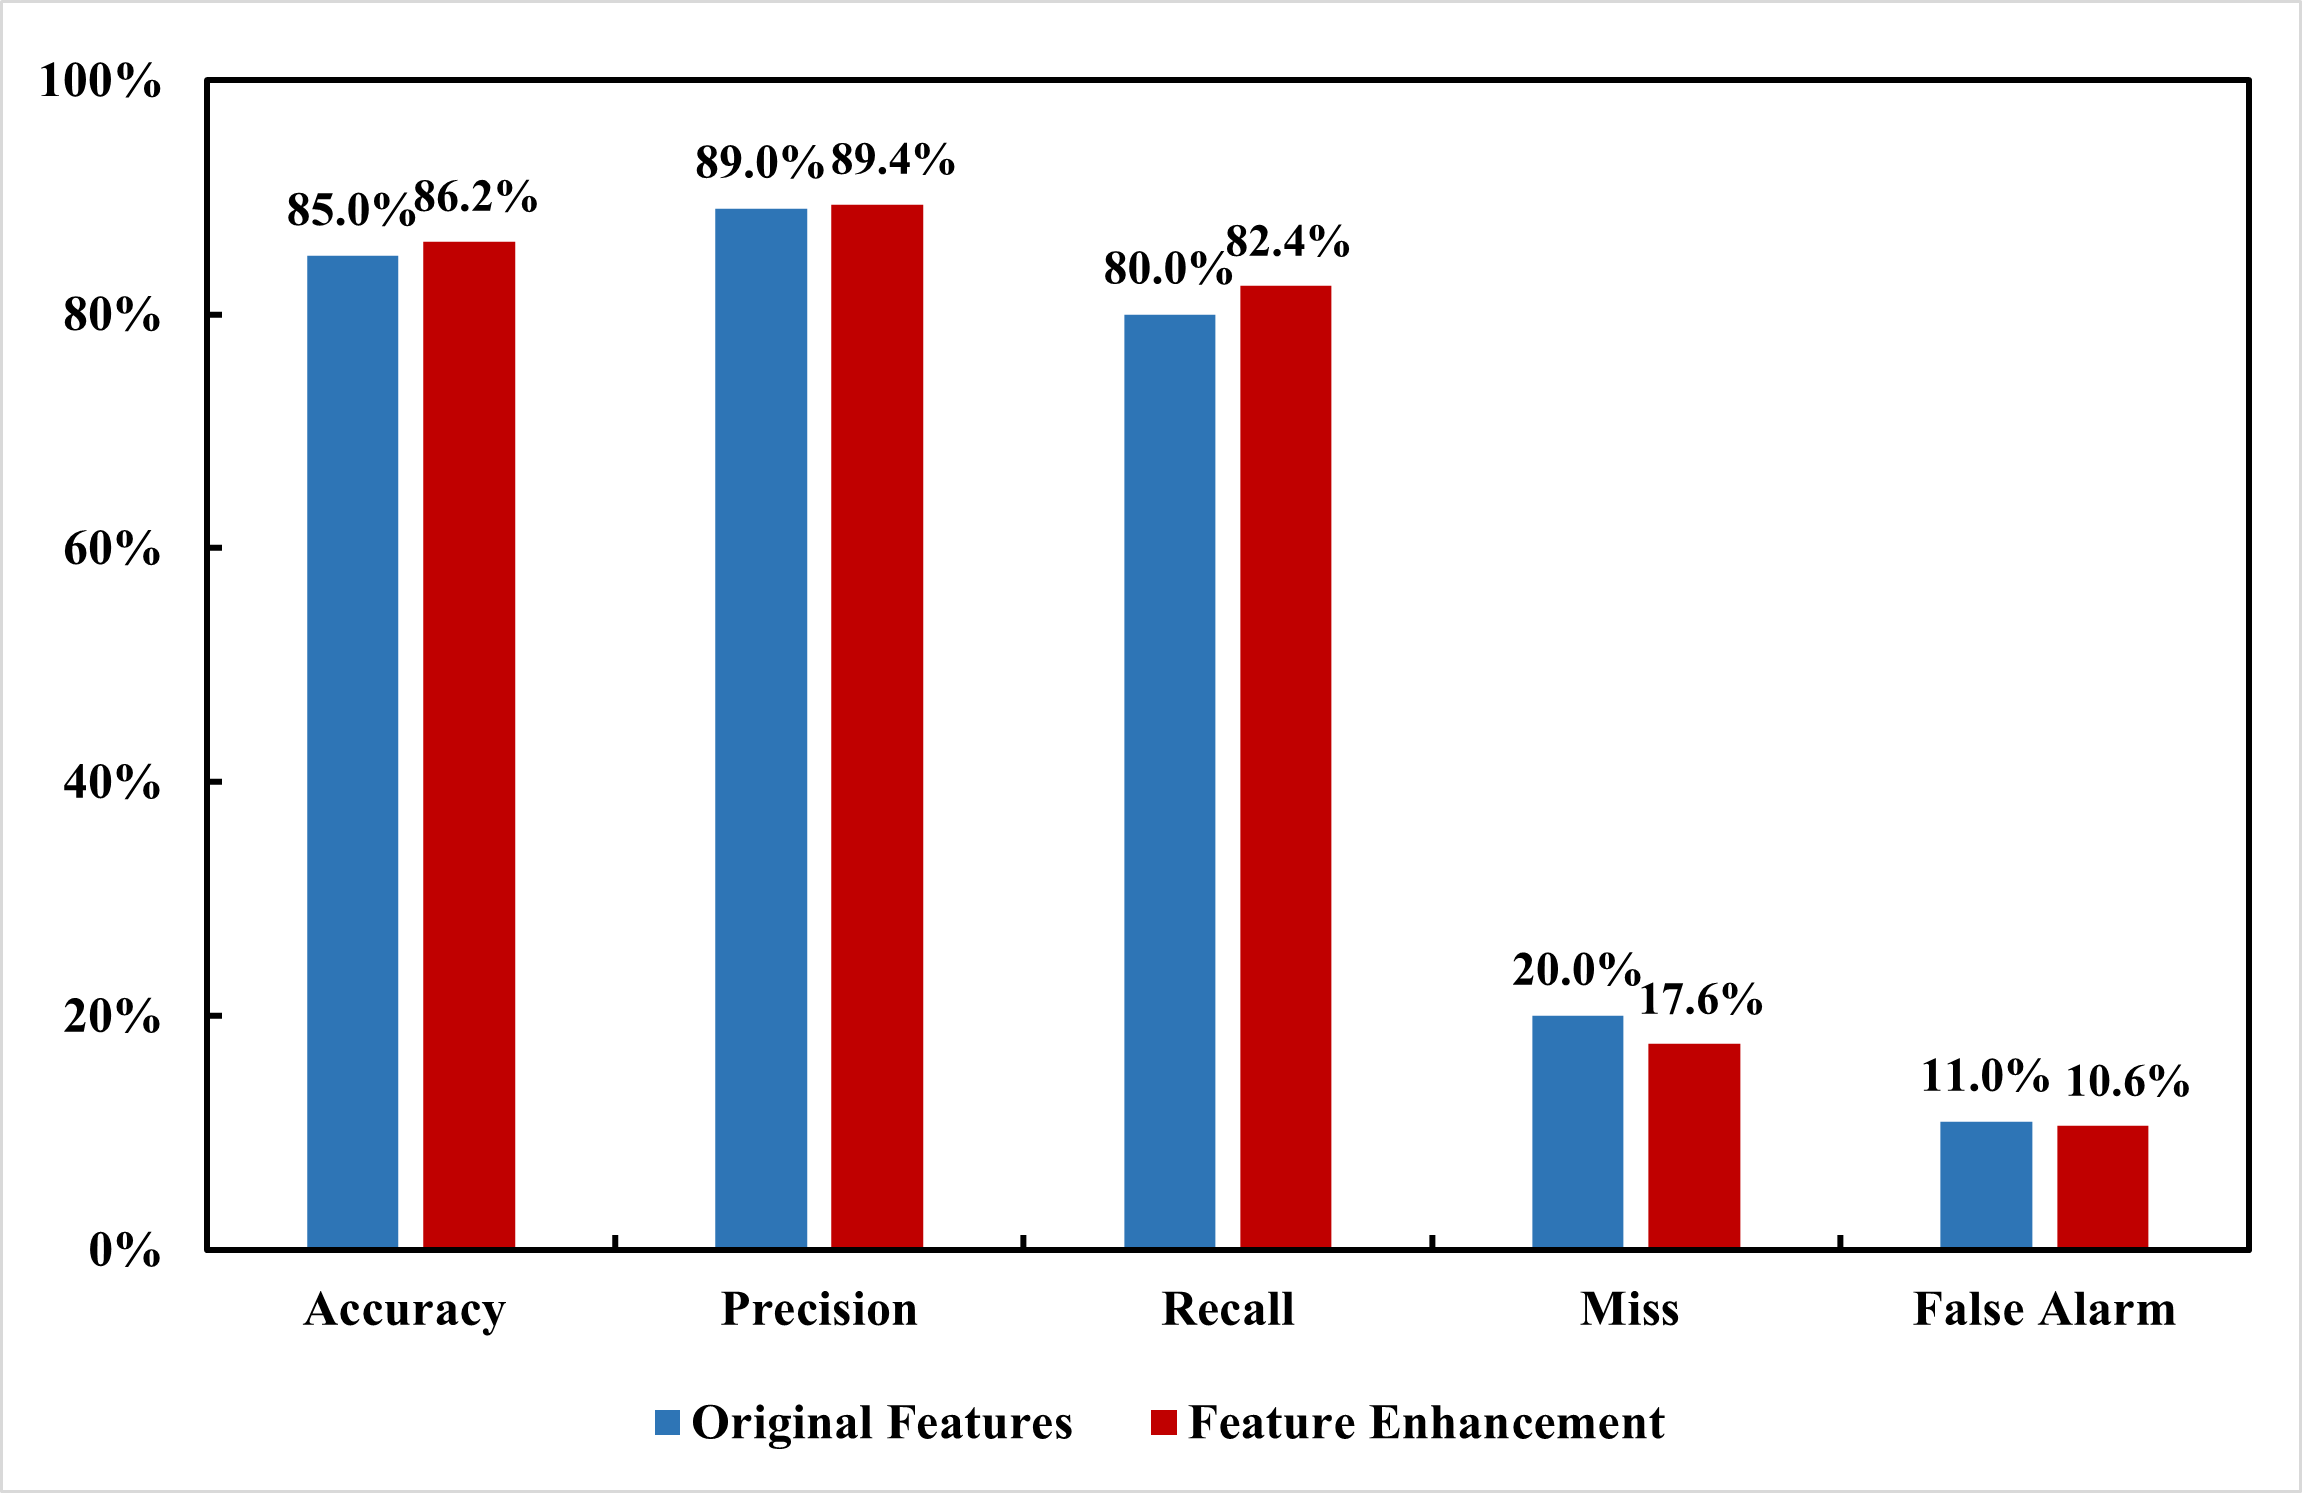
\includegraphics[width=0.75\linewidth]{图片/特征增强.png}
    \caption{Evaluation of feature enhancement effects}
    \label{fig:Evaluation of feature enhancement effects}
\end{figure}

\subsection{Analysis of the effect of data expansion}

As shown in the figure    \label{fig:Analysis of the effect of data expansion} , The findings of this study demonstrate that data expansion significantly improves model performance, especially at 1x and 2x expansion. The increase in accuracy is not significant when the expansion is increased from 2x to 4x. The optimum model performance is achieved with 2x expansion. Expansion beyond 2x is difficult to achieve a full improvement with the current dataset and significantly increases model training time.

\begin{figure}[h]
    \centering
    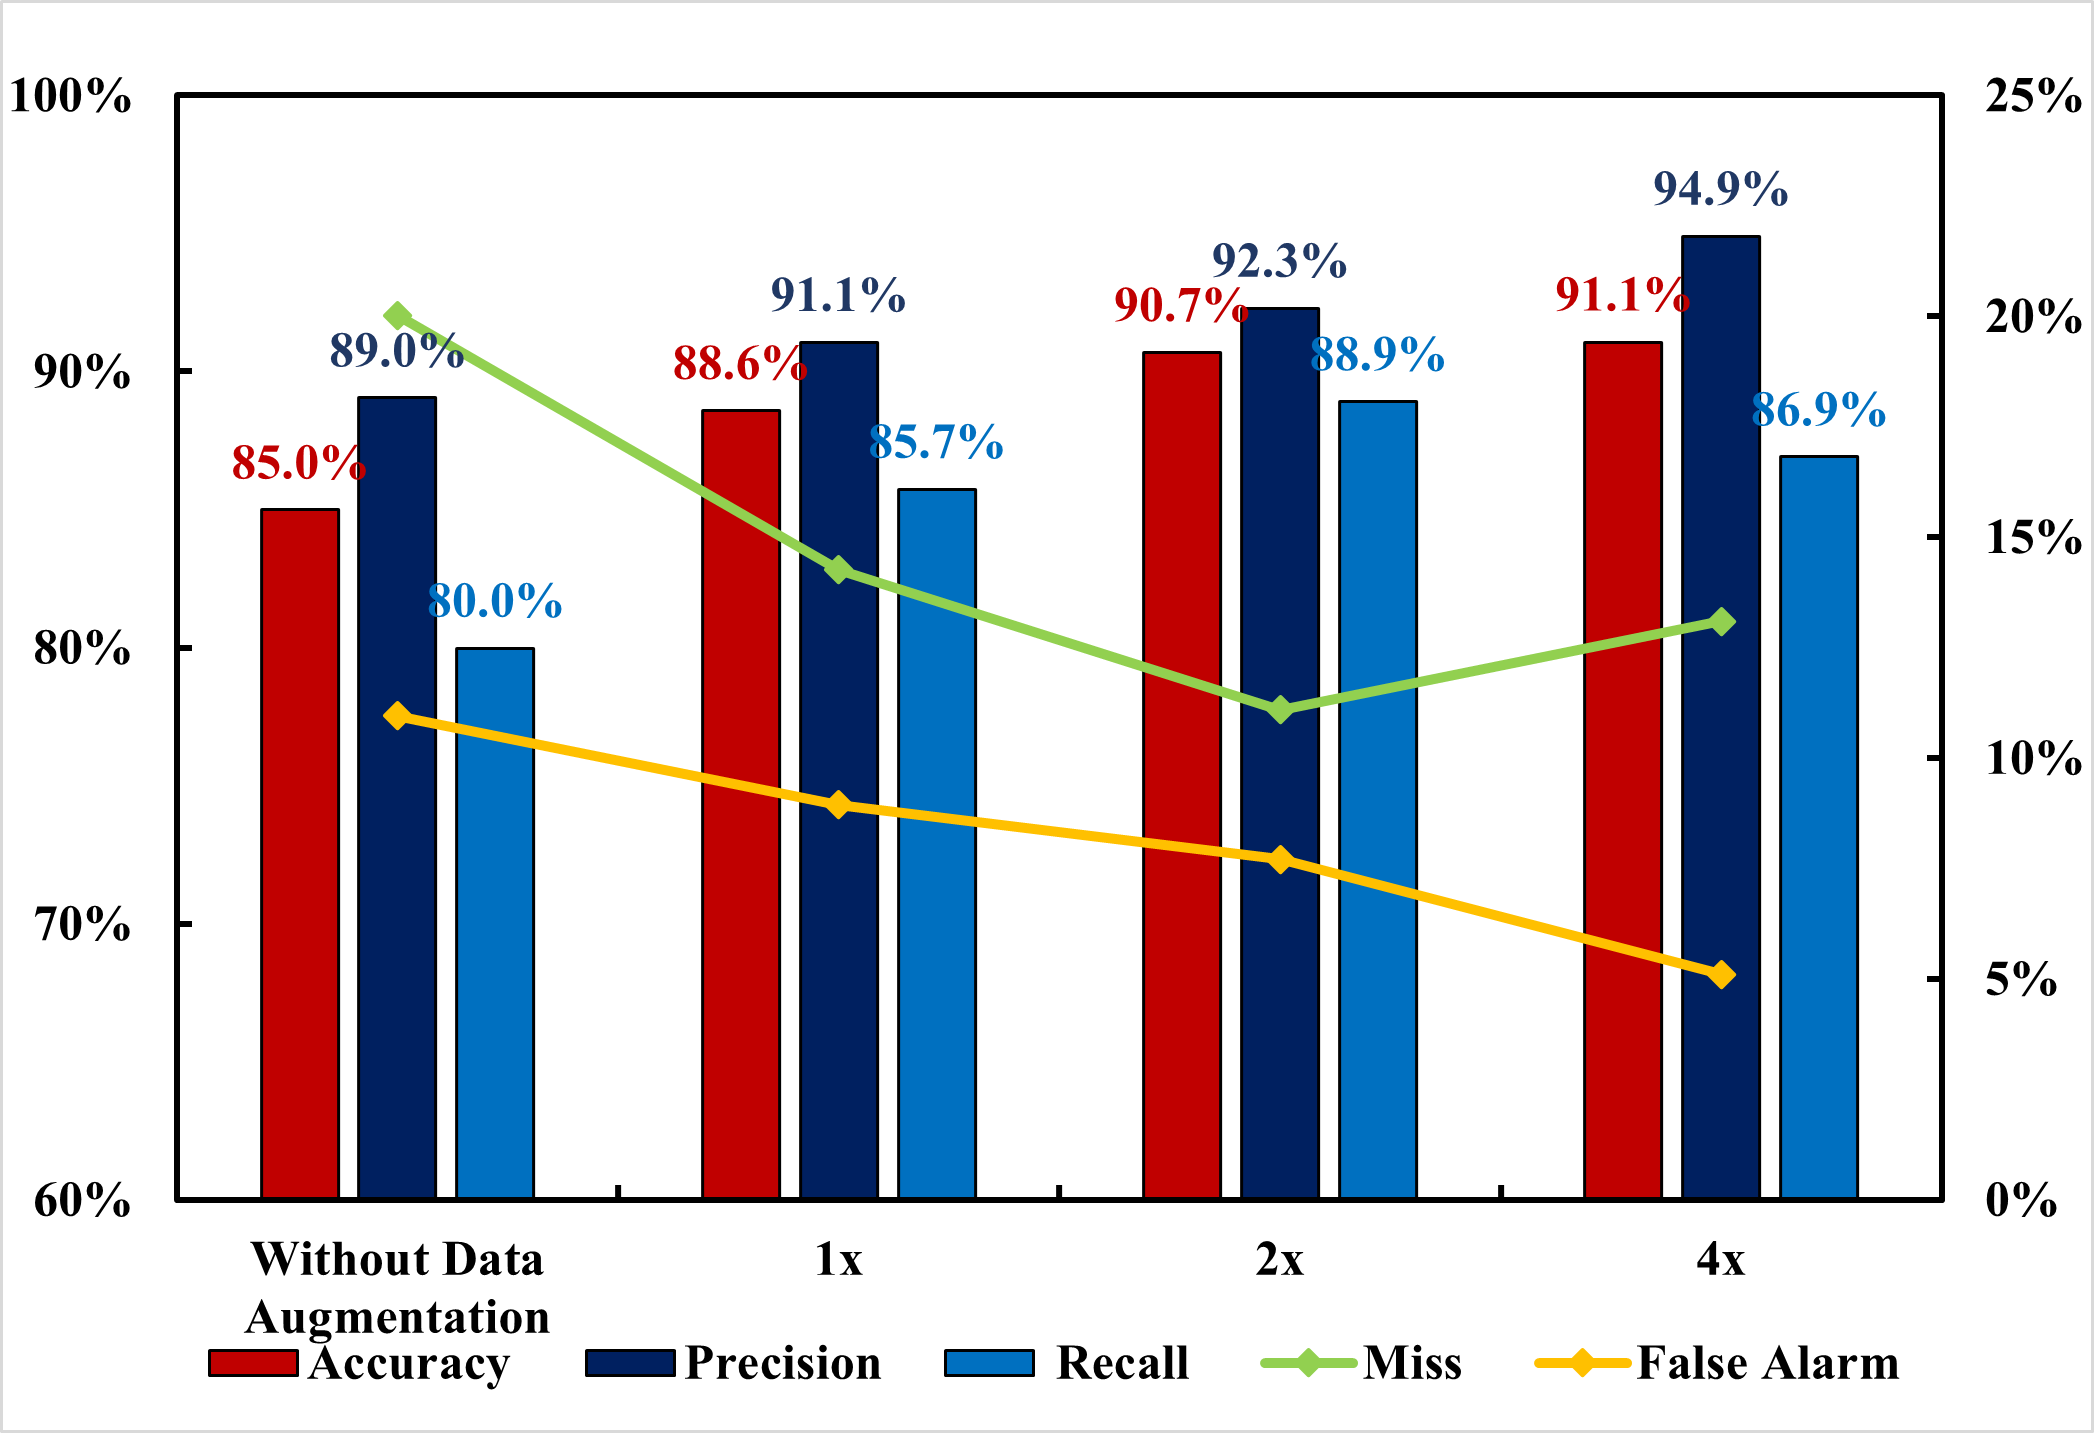
\includegraphics[width=0.75\linewidth]{图片/数据扩充.png}
    \caption{Analysis of the effect of data expansion}
    \label{fig:Analysis of the effect of data expansion}
\end{figure}


%%%%%%%%%%%%%%%%%%%%%%%%%%%%%%%%%%%%%%%%%%
\subsection{Analysis of integrated optimisation effect and multi-scale feature fusion effect}

In the context of the original dataset, which exhibits a loss of circulation, both the feature enhancement method and the data expansion method have been shown to enhance the performance of the model. However, it has been demonstrated that the data expansion method exerts a more substantial influence on the model's performance in comparison to the feature enhancement method. In this study, the two aforementioned methods are fused with multi-scale features, and the effect of multi-scale feature fusion optimisation on model performance is compared with that of individual optimisation, as shown in Figure \label{fig:Comprehensive optimisation effect analysis}. The findings reveal that multi-scale feature fusion optimisation surpasses individual optimisation, attaining an accuracy rate of 93.8\%, a precision rate of 95.1\%, a recall rate of 92.2\%, and leakage and false alarm rates of 7.6\% and 4.8\%, respectively. Following the multi-scale feature fusion, the accuracy and precision of the model have been evidently enhanced in comparison with the unoptimised tandem model. The accuracy has been augmented by 8.8\%, the precision by 6.1\%, the recall by 12.2\%, and the leakage rate by 12.4\%, whilst the false alarm rate has been diminished by 6.2\%.

\begin{figure}[h]
    \centering
    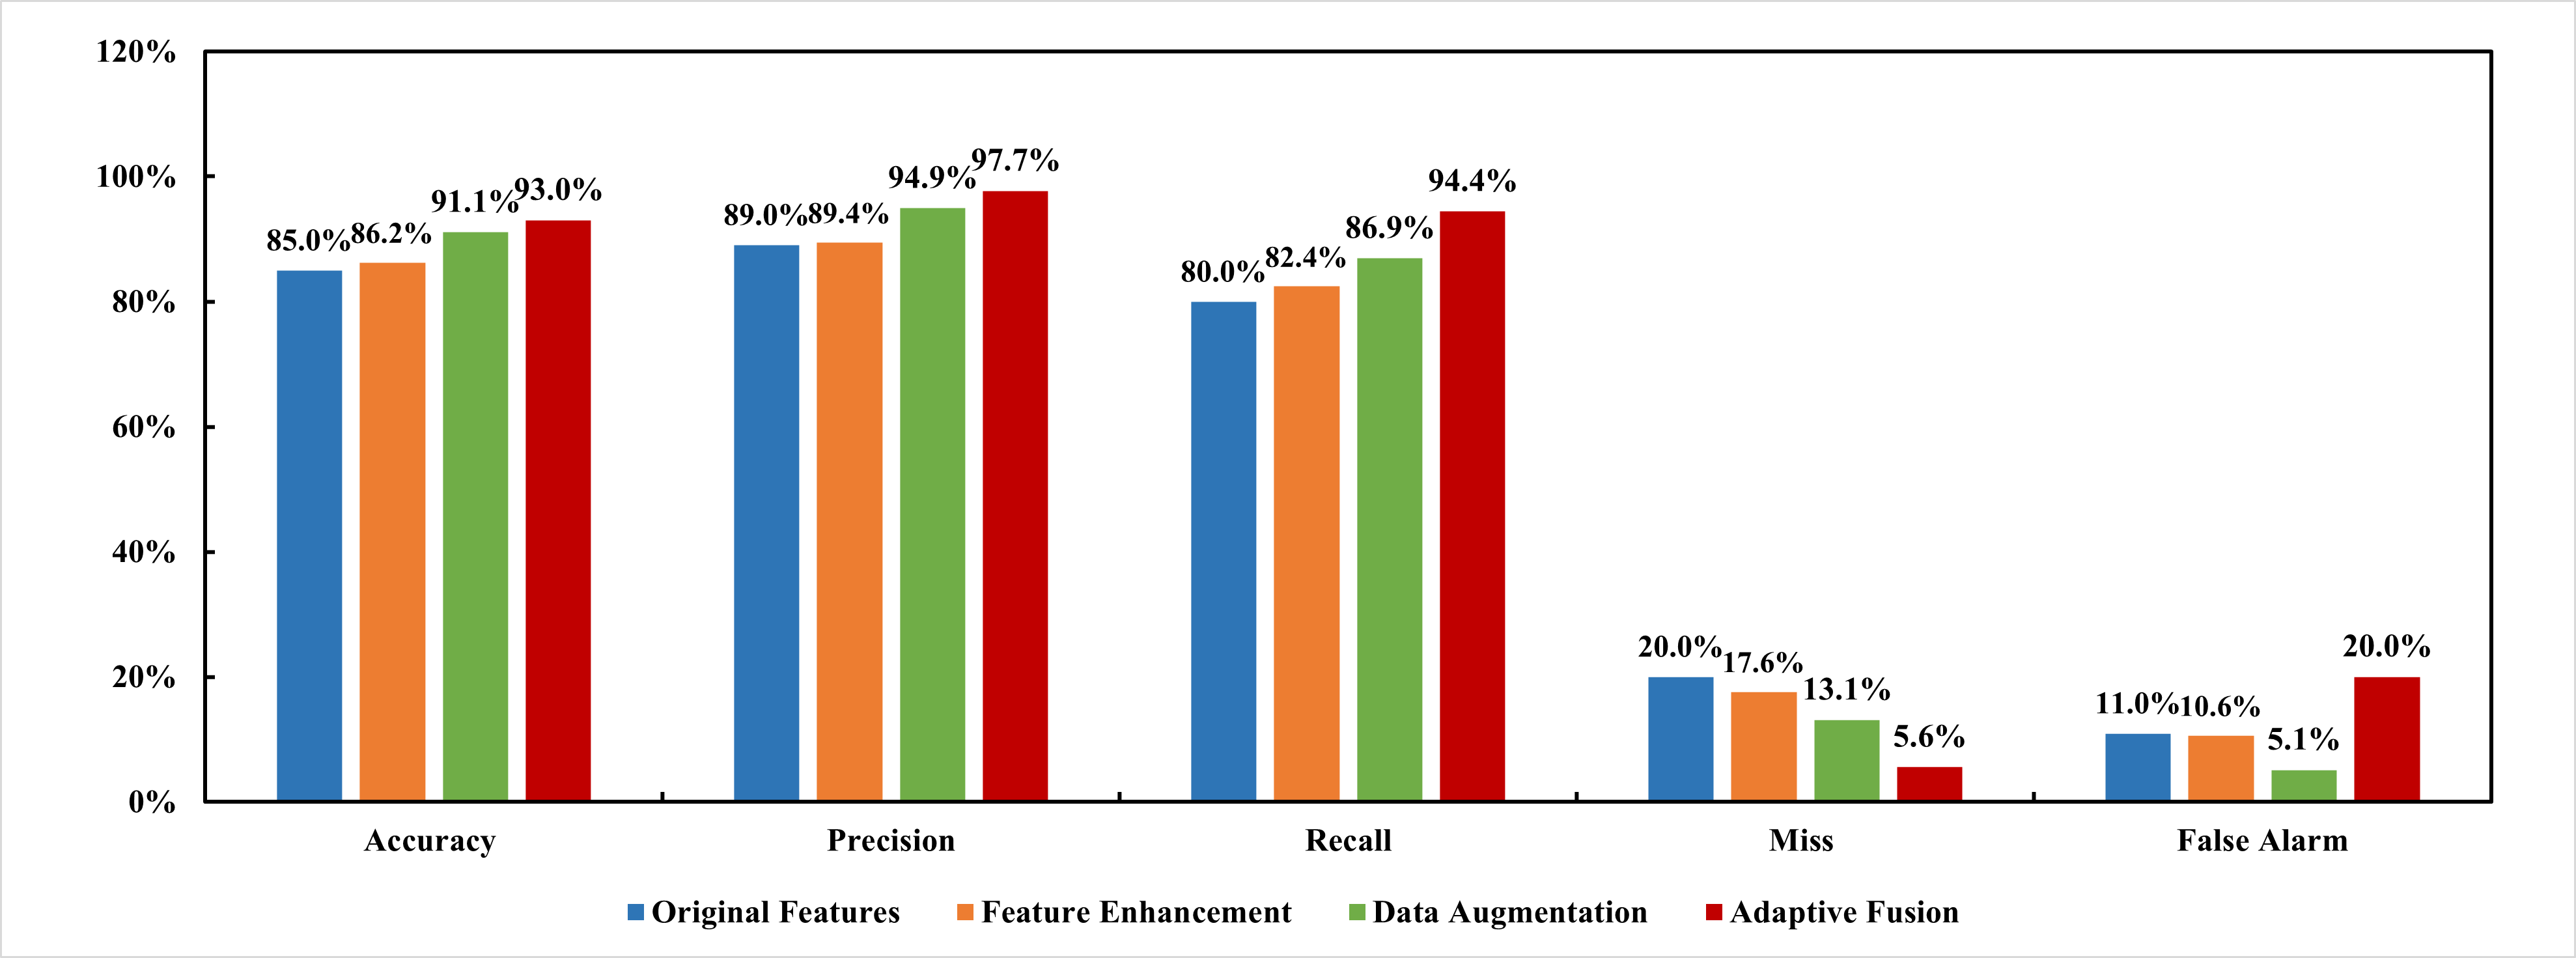
\includegraphics[width=1\linewidth]{图片/综合图像.png}
    \caption{Comprehensive optimisation effect analysis}
    \label{fig:Comprehensive optimisation effect analysis}
\end{figure}
%%%%%%%%%%%%%%%%%%%%%%%%%%%%%%%%%%%%%%%%%%
\section{Conclusion}
The combination of the lost circulation time-series feature enhancement method and time-series data expansion method, in conjunction with the multi-scale feature fusion method, which serves to optimise the stability and generalisation ability of the model, is employed to assess the optimisation effect.

The fusion of feature wavelet transform and genetic programming has been shown to extract effective enhancement features from both deep feature mapping and feature deformation perspectives, thereby significantly improving the diagnostic performance of the model. The model performs optimally with 87.5\% accuracy and 83.4\% recall when the enhanced features of both are used as inputs.

Furthermore, the TimeGAN network has been demonstrated to achieve multidimensional expansion of lost circulation time series data, with the generated data exhibiting a distribution similar to that of the original data. This data expansion has been shown to substantially improve model performance and reduce the occurrence of overfitting. 

With an increase in the expansion multiplier, the model's performance on the test set undergoes a gradual enhancement. When the expansion multiplier is set to 2, the model achieves a balance between performance enhancement and training time, with the accuracy of the test set reaching 90.7\%, the leakage rate at 11.1\%, and the false alarm rate at 7.7\%.

The multi-scale fusion feature approach demonstrates superiority over optimisation alone. The final optimisation result improves the accuracy by 8.8\%, precision by 6.1\%, recall by 12.2\%, and leakage rate and false alarm rate by 12.4\% and 6.2\%, respectively, compared with the unoptimised model.


%%%%%%%%%%%%%%%%%%%%%%%%%%%%%%%%%%%%%%%%%%


\begin{adjustwidth}{-\extralength}{0cm}

\reftitle{References}

\bibliography{ref}


\vspace{20pt} 

\noindent \textbf{Disclaimer/Publisher’s Note:} The statements, opinions and data contained in all publications are solely those of the individual author(s) and contributor(s) and not of MDPI and/or the editor(s). MDPI and/or the editor(s) disclaim responsibility for any injury to people or property resulting from any ideas, methods, instructions or products referred to in the content.


\end{adjustwidth}




%%%%%%%%%%%%%%%%%%%%%%%%%%%%%%%%%%%%%%%%%%


\end{document}

